%%==========================================================================
\section{Experiments}
\label{sec:experiments}

We have used synthetically generated data as well as real captured data to evaluate the SuperMatching algorithm.
To demonstrate the independence and generalization of the SuperMatching, different descriptors have been applied.
For 2D deformable surface, the SIFT features~\cite{Lowe04} are used.
While for the 3D shapes without color information, the spin images features~\cite{Johnson99} are employed.
For the 3D colorful shapes, both SIFT and spin images are employed.
To build the matching between two shapes, we used third-order matching for the experiment.
For the multiple scanned shapes (number is $n$), 
the third-order matching is first performed between two consecutive frames, 
then global optimization with $max(n/4,3)$th higher-order matching in the slices (with n/5 frames) of the whole sequences.

%-------------------------------------------------------------------------
\subsection{2D deformable surfaces}
\label{subsec:2ddeformabledata}

Firstly, we used a 2D deformable surface data \footnote{From \url{http://cvlab.epfl.ch/data/dsr/}} with a cloth and a cushion.
The surfaces of the cloth underwent relatively smooth deformations, while the surfaces of the cushion included sharp folds.
The data has provided ground truth, which are very useful to to verify the accuracy of our method quantitatively.
From each image set we randomly chose six frames before and after a large deformation. 
We randomly chose $100$ corresponding points on each surface to be the features, using the provided ground truth.
In each image set we chose the features on the frame most unlike the others  (shown in Fig.\ref{fig:mini:subfig_deformableimages}) 
as $P_1$ and matched them with the features in the other five frames.

We chose the data as a basis for comparison the spectral algorithm~\cite{Cour06} (a pairwise algorithm),
a third-order tensor algorithm~\cite{Duchenne09},
and the hyper graph matching algorithm~\cite{Zass08}, using the authors' code in each case.
All methods were executed in Matlab on a $2.3$GHz Core2Duo with $2$GB memory.
To enable direct and fair comparison, 
~\cite{Duchenne09}, ~\cite{Zass08} and our method used the same potential and all maintained an equivalent tensor size.

In the test our method used $20000$ feature tuples, while the method of~\cite{Duchenne09} used 1010000 features  and the method of~\cite{Zass08} used $40000$.
The average running time to match two feature sets each with $100$ features was around 8s for our method, 13s for \cite{Duchenne09}, 6.5s for~\cite{Zass08}, and $5$s for~\cite{Cour06}.
As we use the same tensor size but sample fewer feature tuples, we achieve a higher matching accuracy with less computation than third-order tensor algorithm~\cite{Duchenne09}.

The matching accuracy is given as the number of correctly matched points (according to the provided ground truth) divided by the total number of points that could potentially be matched. 
The results for all methods, using the two image sets, are given in Tables~\ref{tab:errorrate1} and~\ref{tab:errorrate2} and are illustrated in Fig.\ref{fig:mini:deformablematchingimages}. 
Our method matched all the features on the deforming surfaces, while others did not.

%----------------------------------------
%  deformable matching : model features
%----------------------------------------
\begin{figure*}[!t]
%\vspace{-4mm}
%\hspace{-8ex}
%\setlength{\abovecaptionskip}{2mm}
%\setlength{\belowcaptionskip}{2mm}
\renewcommand\thesubfigure{}
\centering
\setlength\subfigcapskip{-4mm}
%\vspace{-2ex}
        \hspace{-8ex}
        \begin{minipage}[b]{0.2\textwidth}
            \subfigure[\scriptsize Frame 299]{
            \label{fig:subfig:cloth1}
            \centering
            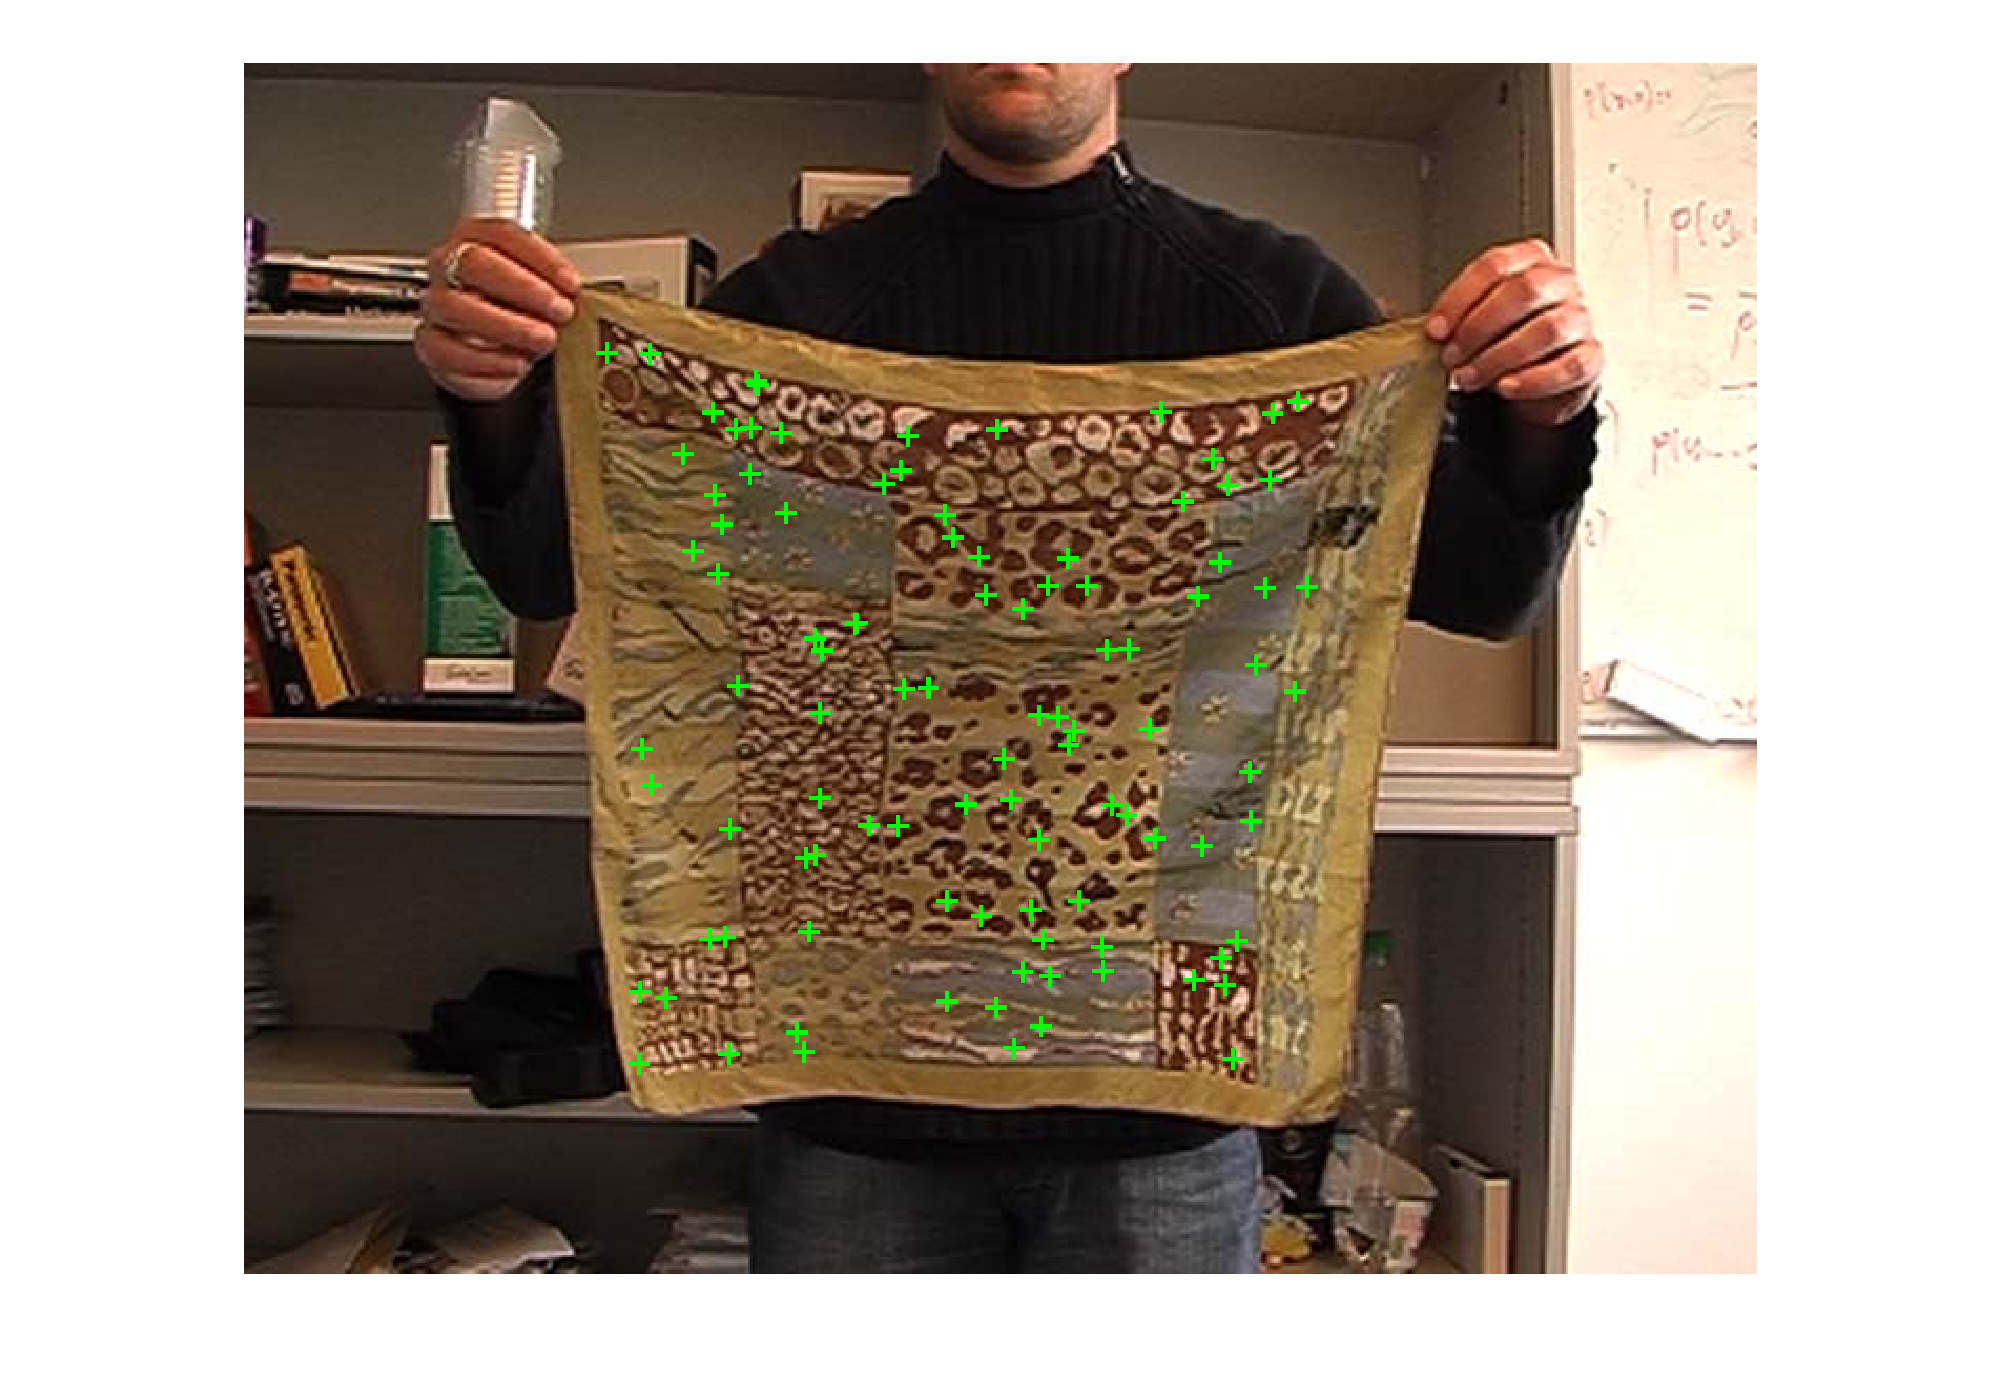
\includegraphics[width=36mm]{cloth_299.pdf}}%
        \end{minipage}%
        \hspace{5mm}%
        \addtocounter{subfigure}{-1}
        %%%
        \begin{minipage}[b]{0.2\textwidth}
            \subfigure[\scriptsize Frame 314]{
            \label{fig:subfig:paperB1}
            \centering
            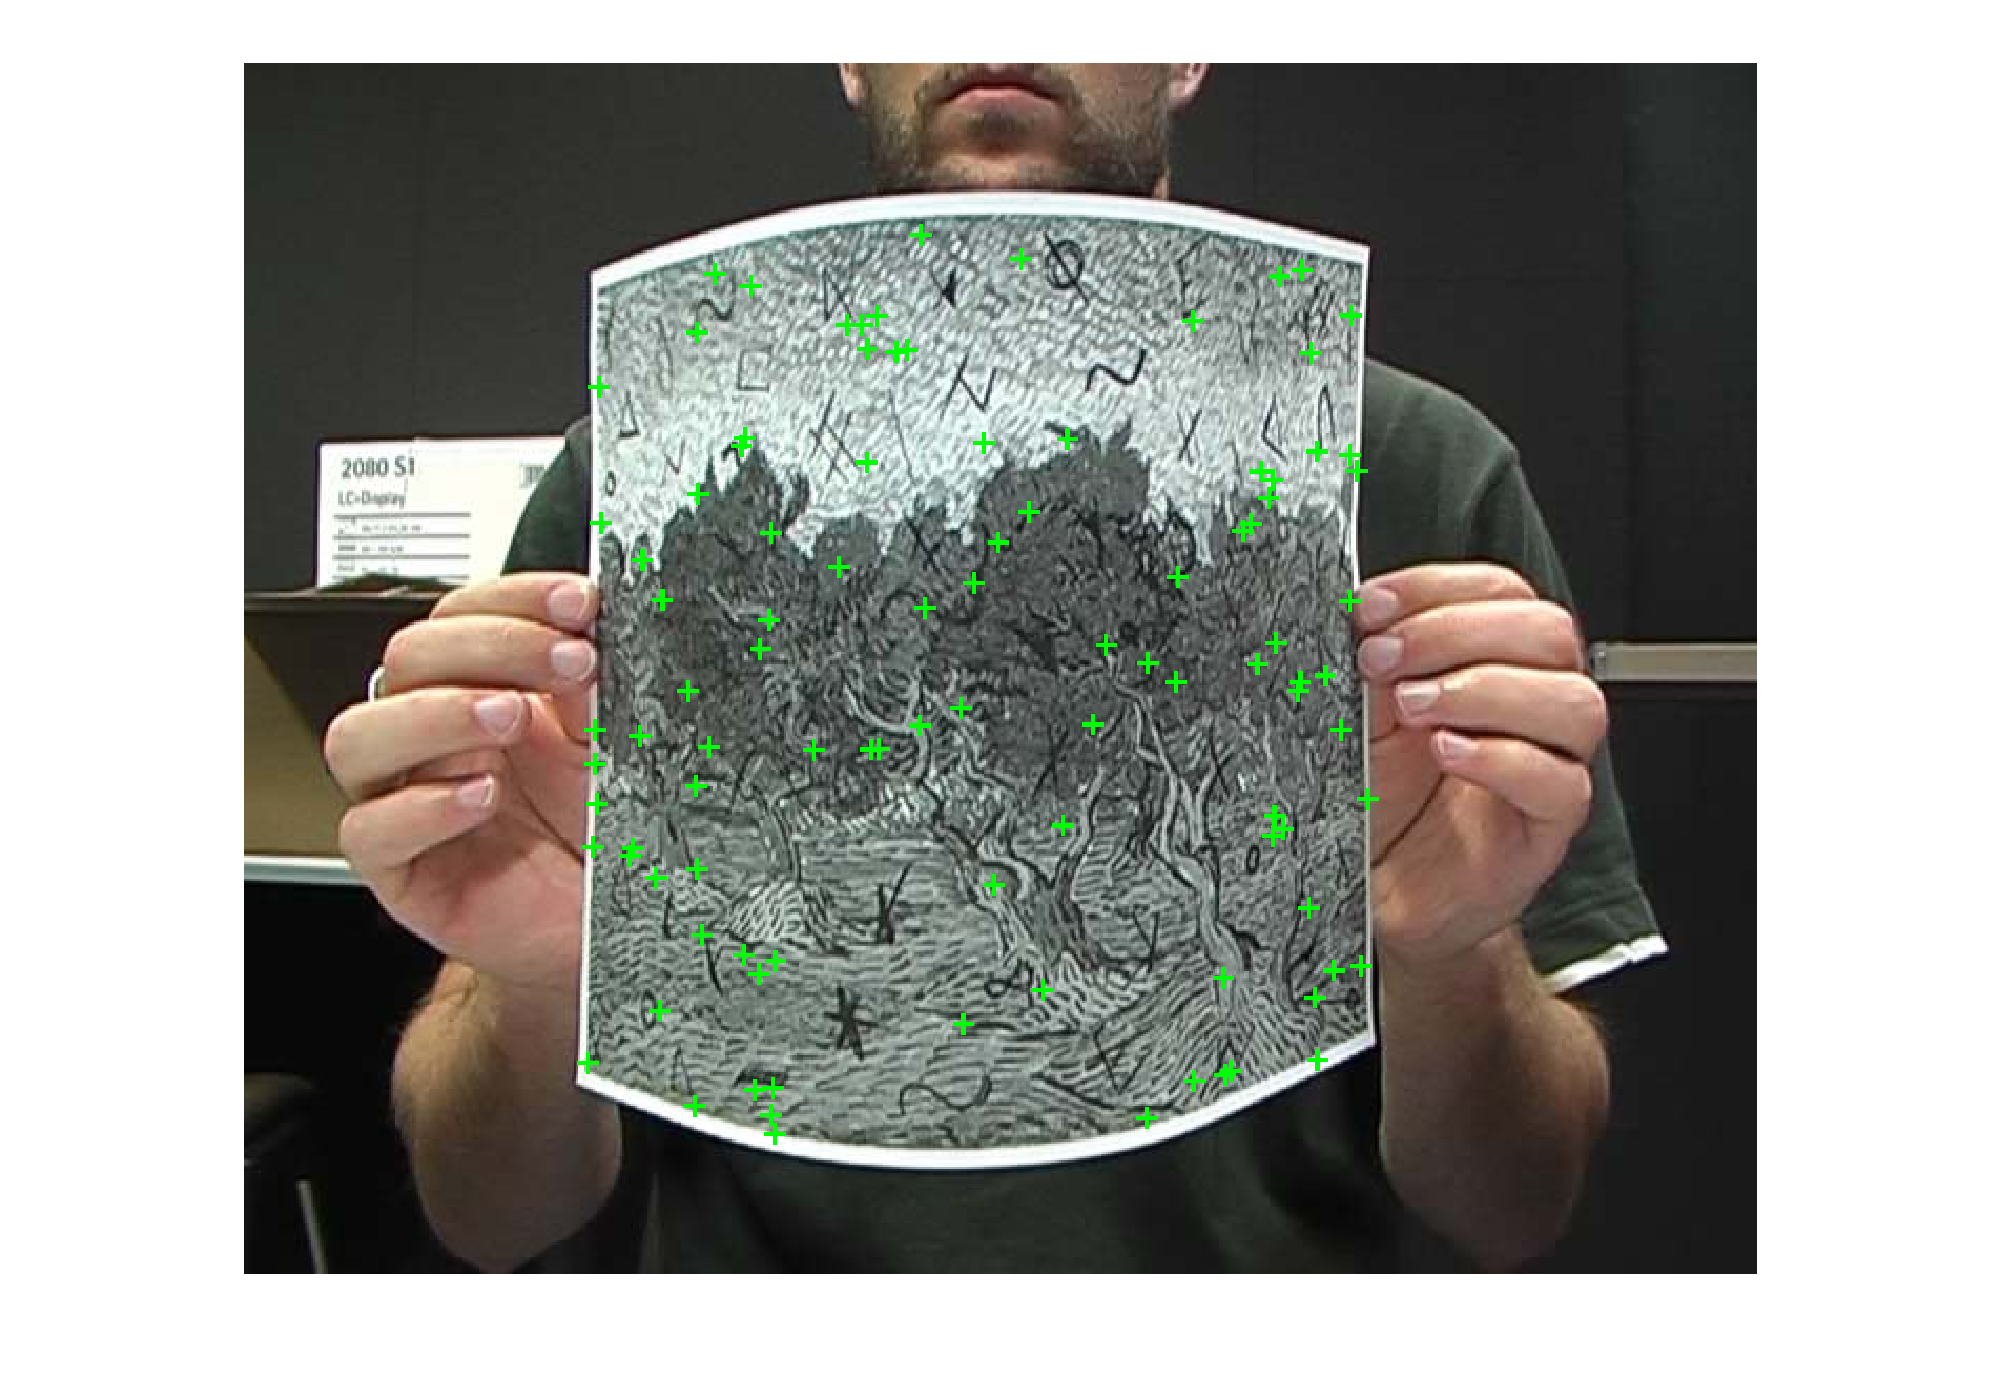
\includegraphics[width=36mm]{paperB_314.pdf}}%
        \end{minipage}%
        \hspace{5mm}%
        \addtocounter{subfigure}{-1}
        %%%
        \begin{minipage}[b]{0.2\textwidth}
            \subfigure[\scriptsize Frame 213]{
            \label{fig:subfig:cushion1}
            \centering
            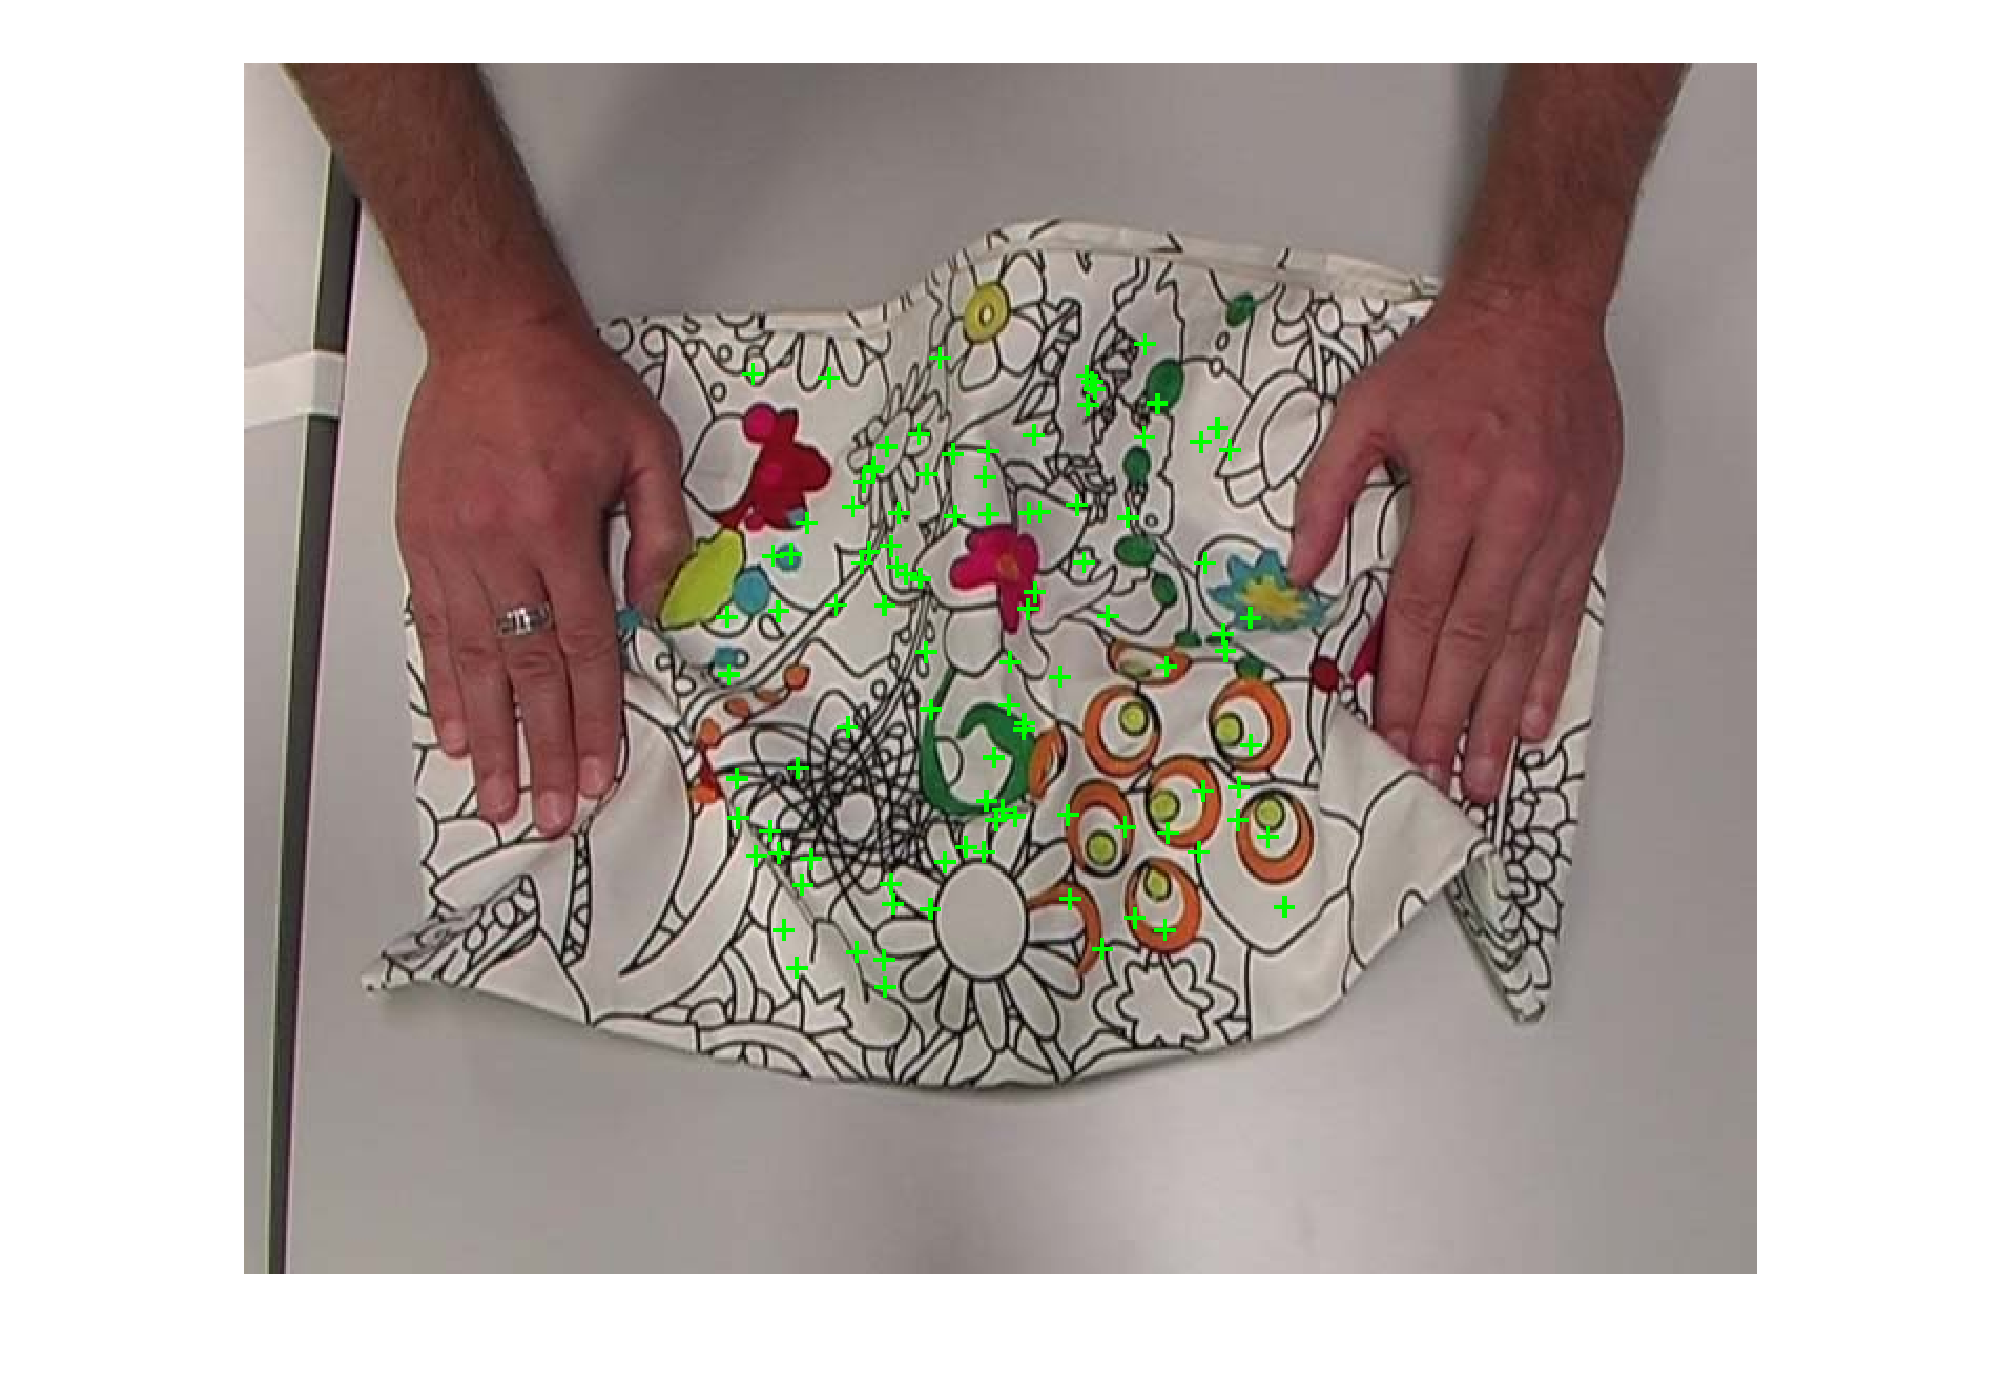
\includegraphics[width=36mm]{cushion_213.pdf}}%
        \end{minipage}%
        \hspace{5mm}%
        \addtocounter{subfigure}{-1}
        %%%
        \begin{minipage}[b]{0.2\textwidth}
            \subfigure[\scriptsize Frame 375]{
            \label{fig:subfig:paperc1}
            \centering
            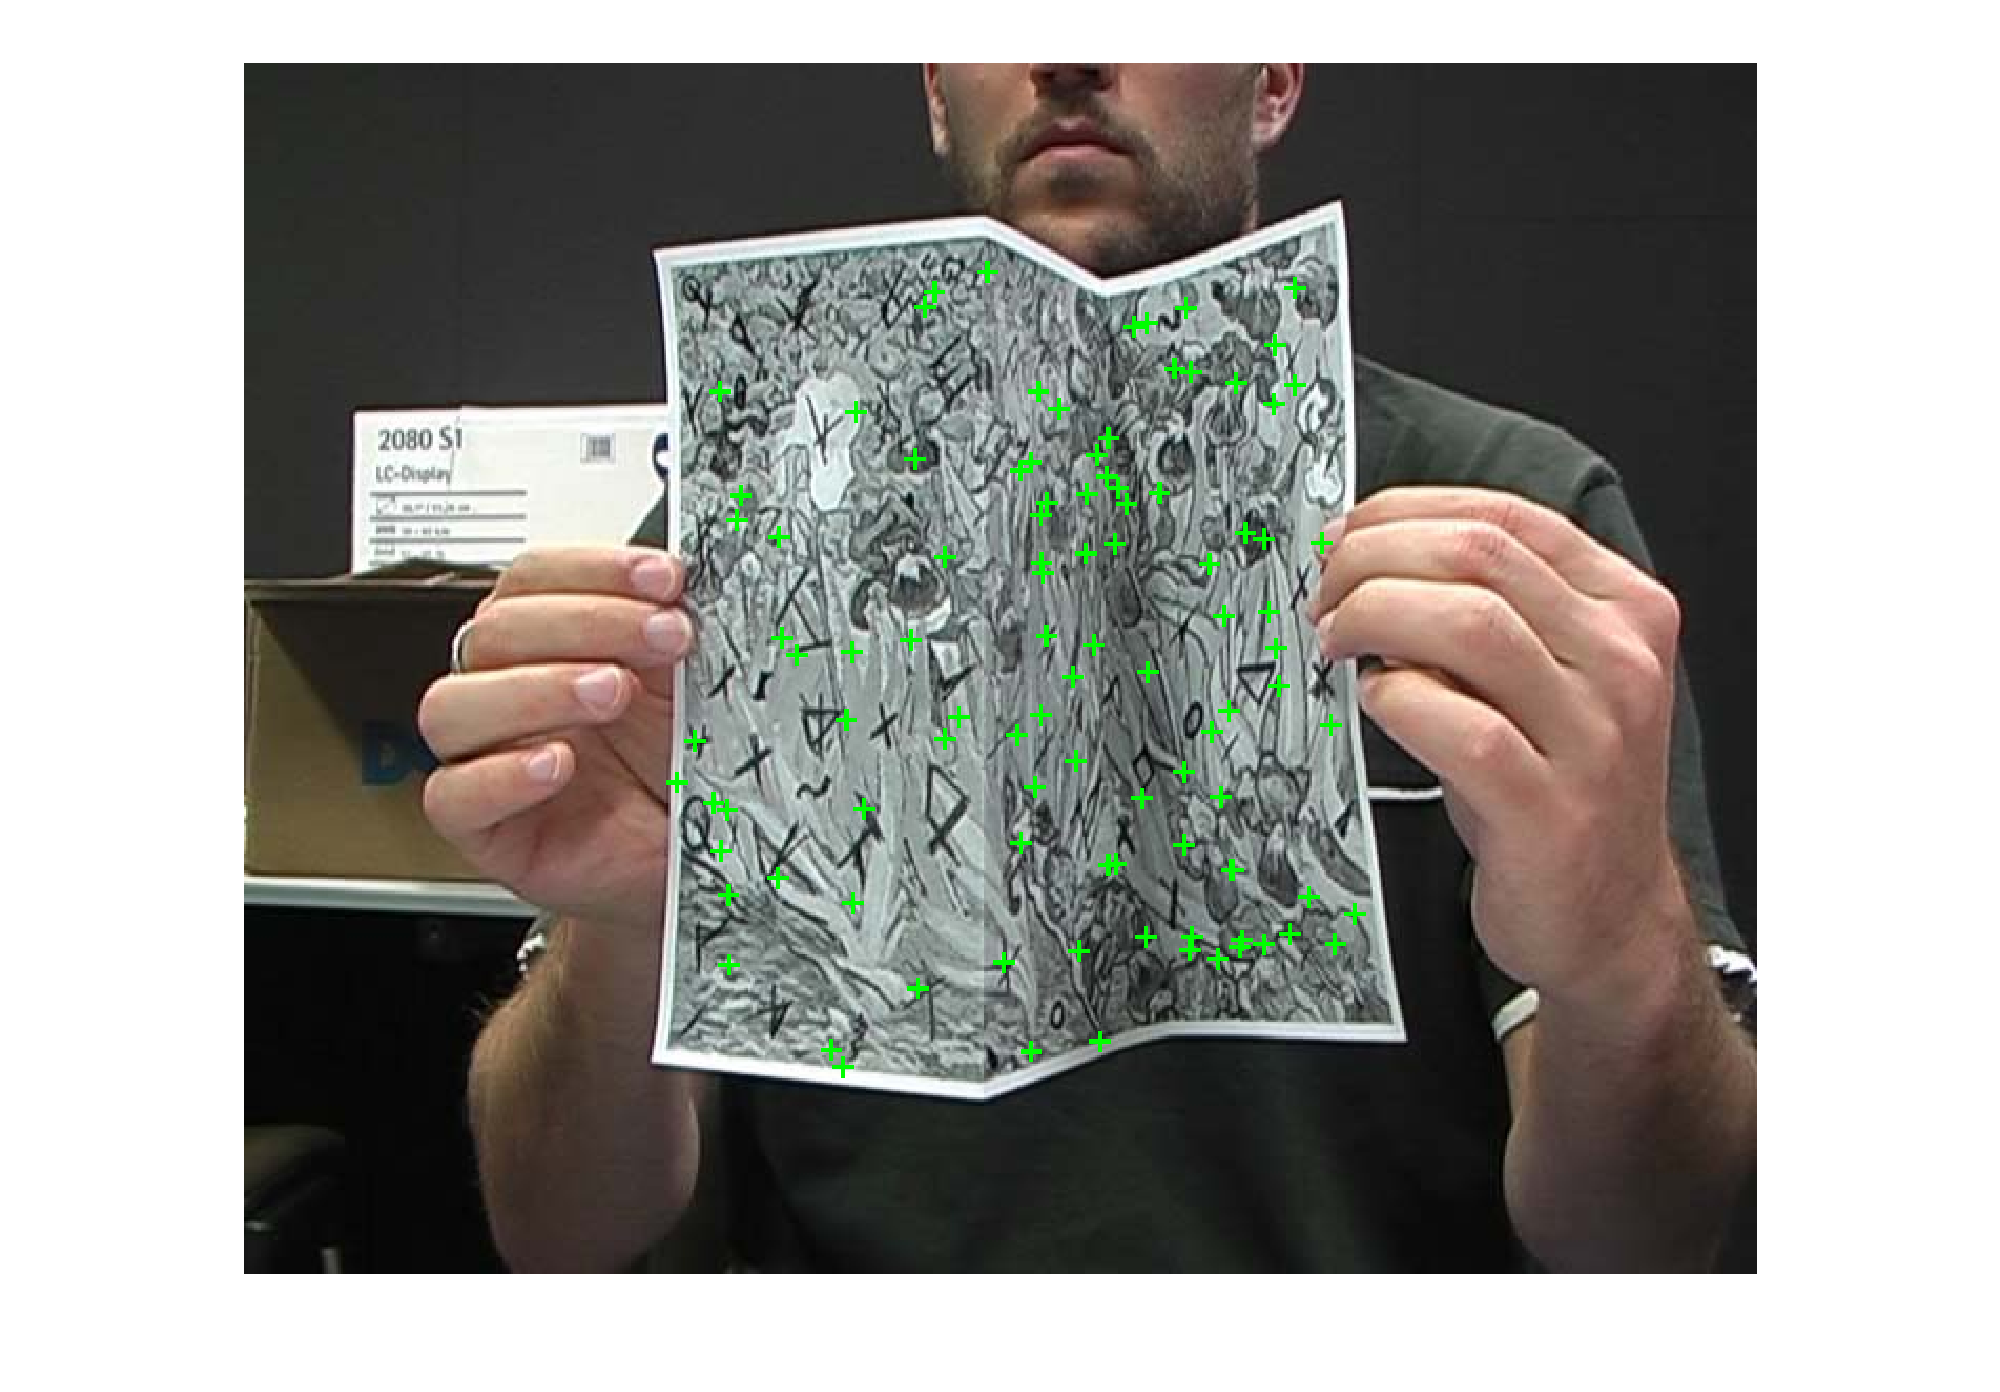
\includegraphics[width=36mm]{paperC_375.pdf}}%
        \end{minipage}\\%
        %\hspace{22mm}%
        \addtocounter{subfigure}{-1}
        \caption{Left to right: point sets on the surface of a piece of cloth, a piece of smoothly curving paper, a creased cushion and a piece of creased paper. The frame number is below each image. }
\label{fig:mini:subfig_deformableimages} %% label for entire figure
\end{figure*}%
%----------------------------------------
%  deformable matching results IMAGES
%----------------------------------------
\begin{figure*}[!ht]
\setlength{\abovecaptionskip}{0mm}
\setlength{\belowcaptionskip}{-4mm}
\centering
\setlength\subfigcapskip{-2mm}
%\vspace{-2ex}
        \hspace{-8ex}
         %----------------------------
         %%% smac method
         %----------------------------
        \begin{minipage}[b]{0.4\textwidth}
        \subfigure{
            \label{fig:subfig:clothmatching1}
            \centering
            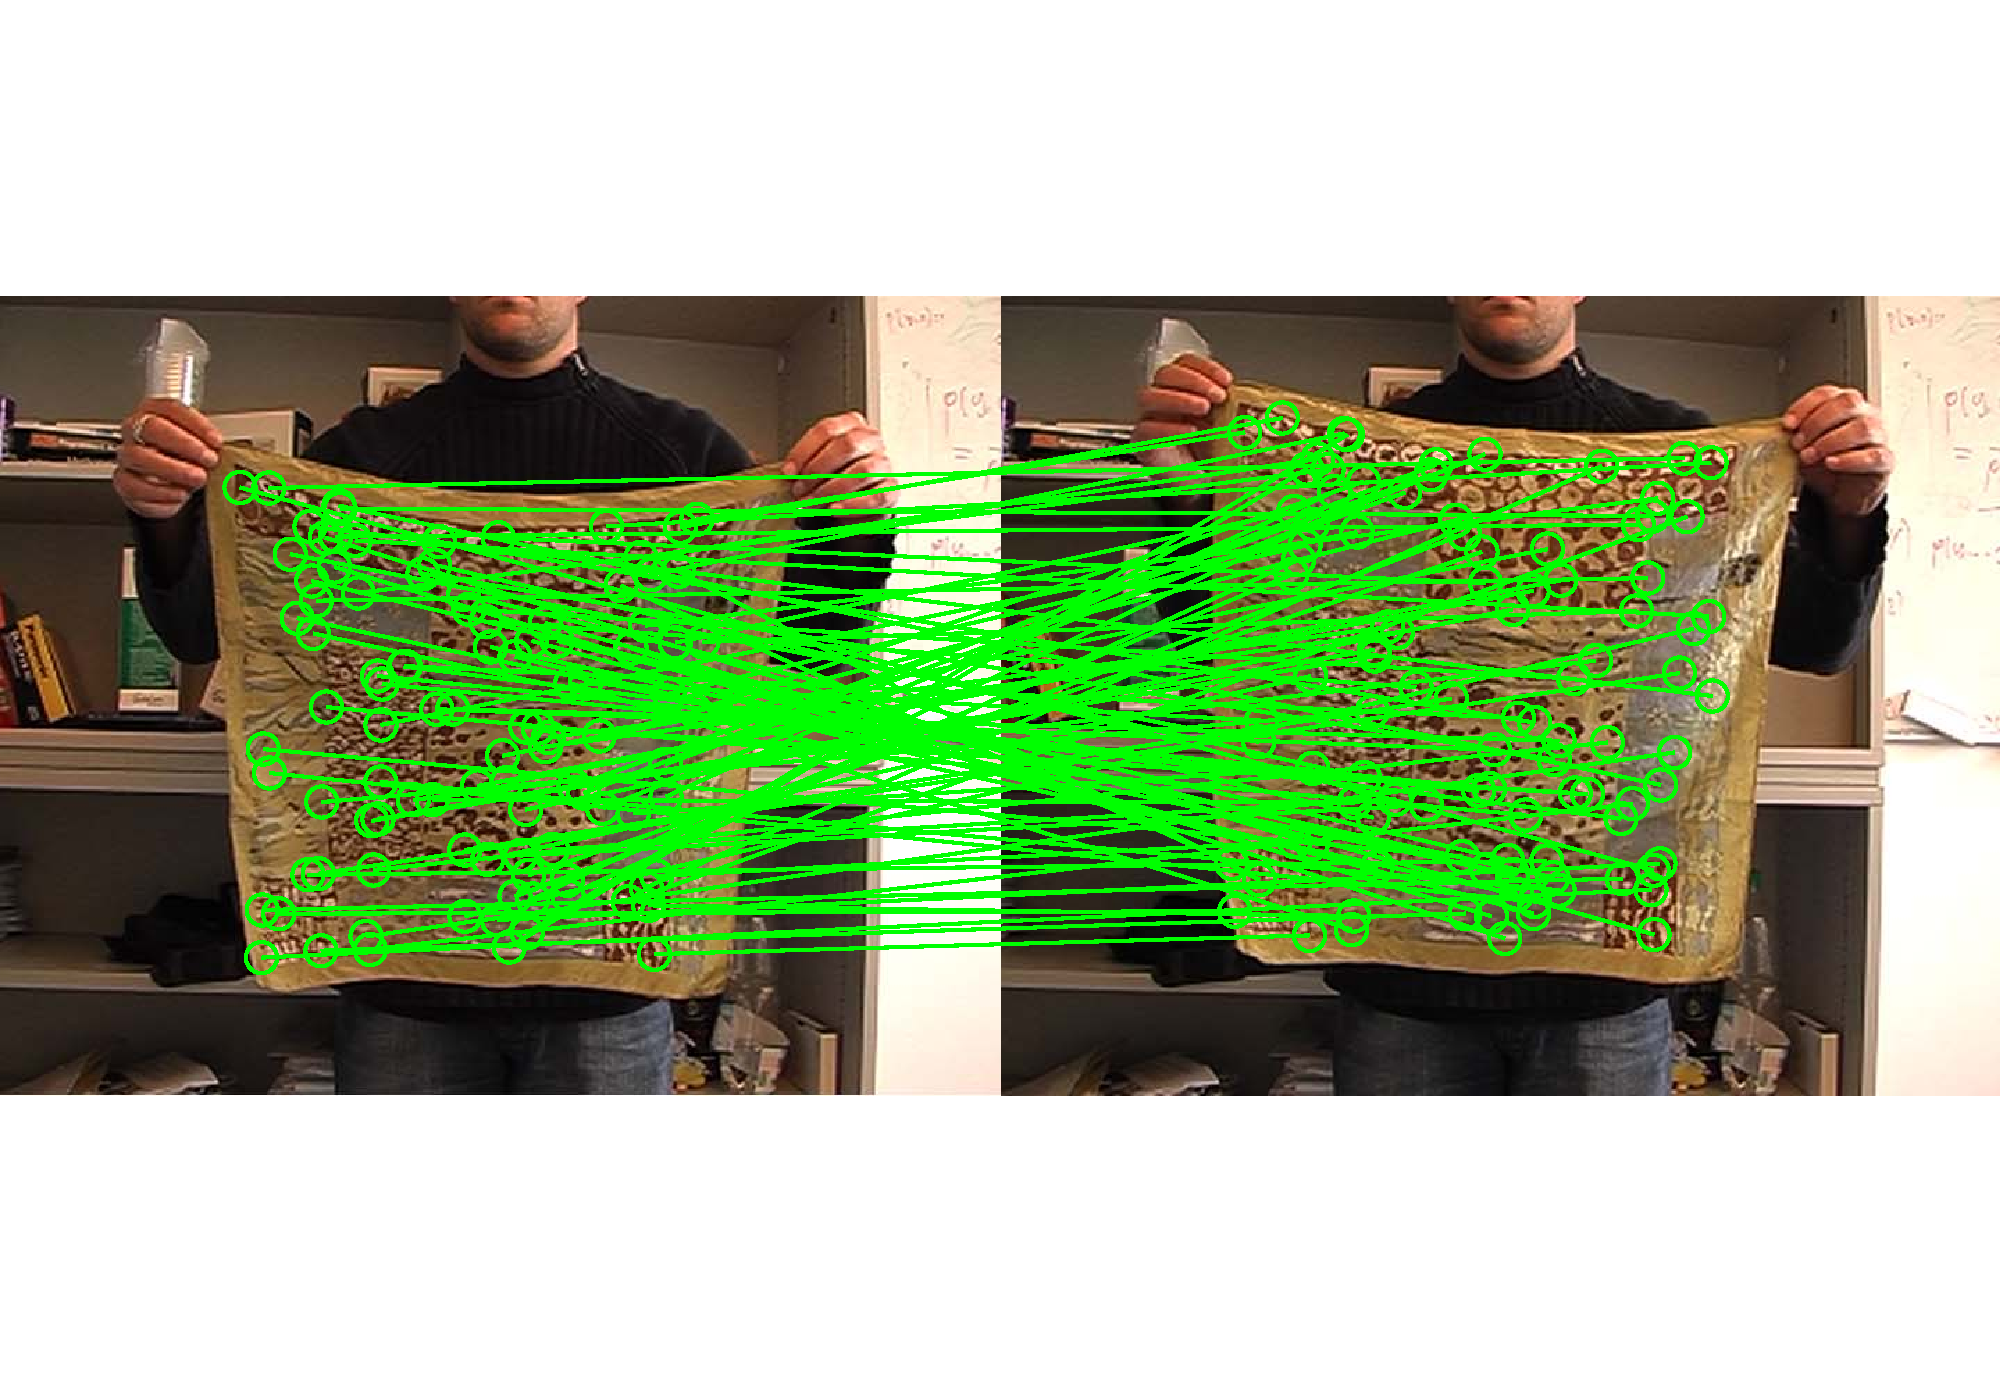
\includegraphics[width=62mm]{SMAC_F258-F299.pdf}%
            }%
        \end{minipage}%
        \hspace{8mm}%
        \addtocounter{subfigure}{-1}
        %%%
        \begin{minipage}[b]{0.4\textwidth}
        \subfigure{
            \label{fig:subfig:clothmatching2}
            \centering
            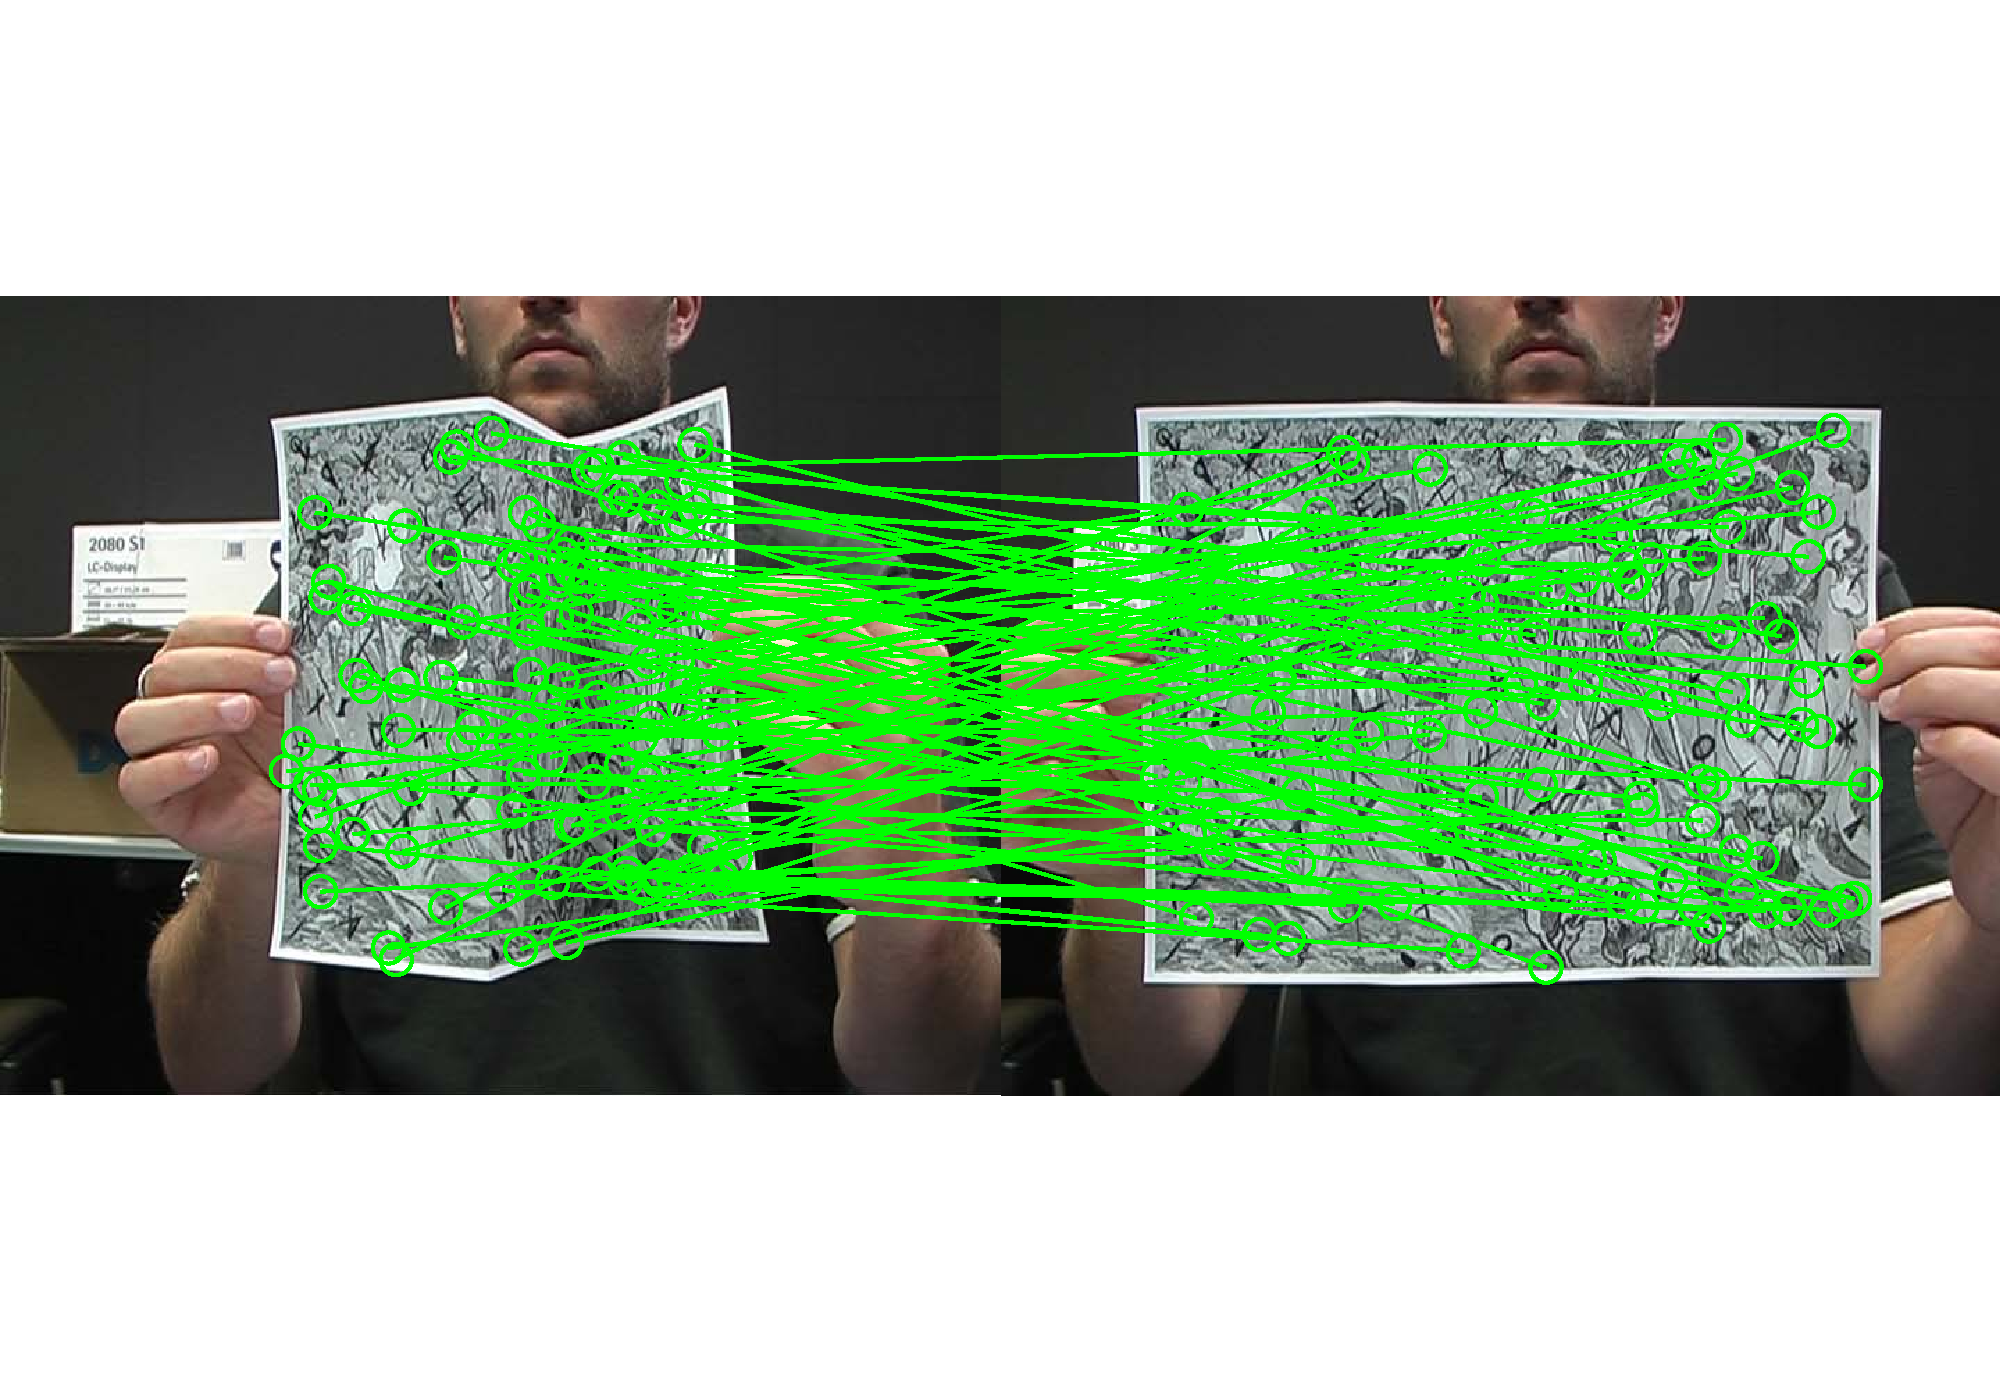
\includegraphics[width=60mm]{SMAC_F309-375.pdf}%
            }%
        \end{minipage}\\%
        %\hspace{28mm}%
        \addtocounter{subfigure}{-1}%
        %----------------------------
        %%% HYPER method
        %----------------------------
        \hspace{-8ex}
        \begin{minipage}[b]{0.4\textwidth}
        \subfigure{
            \label{fig:subfig:clothmatching3}
            \centering
            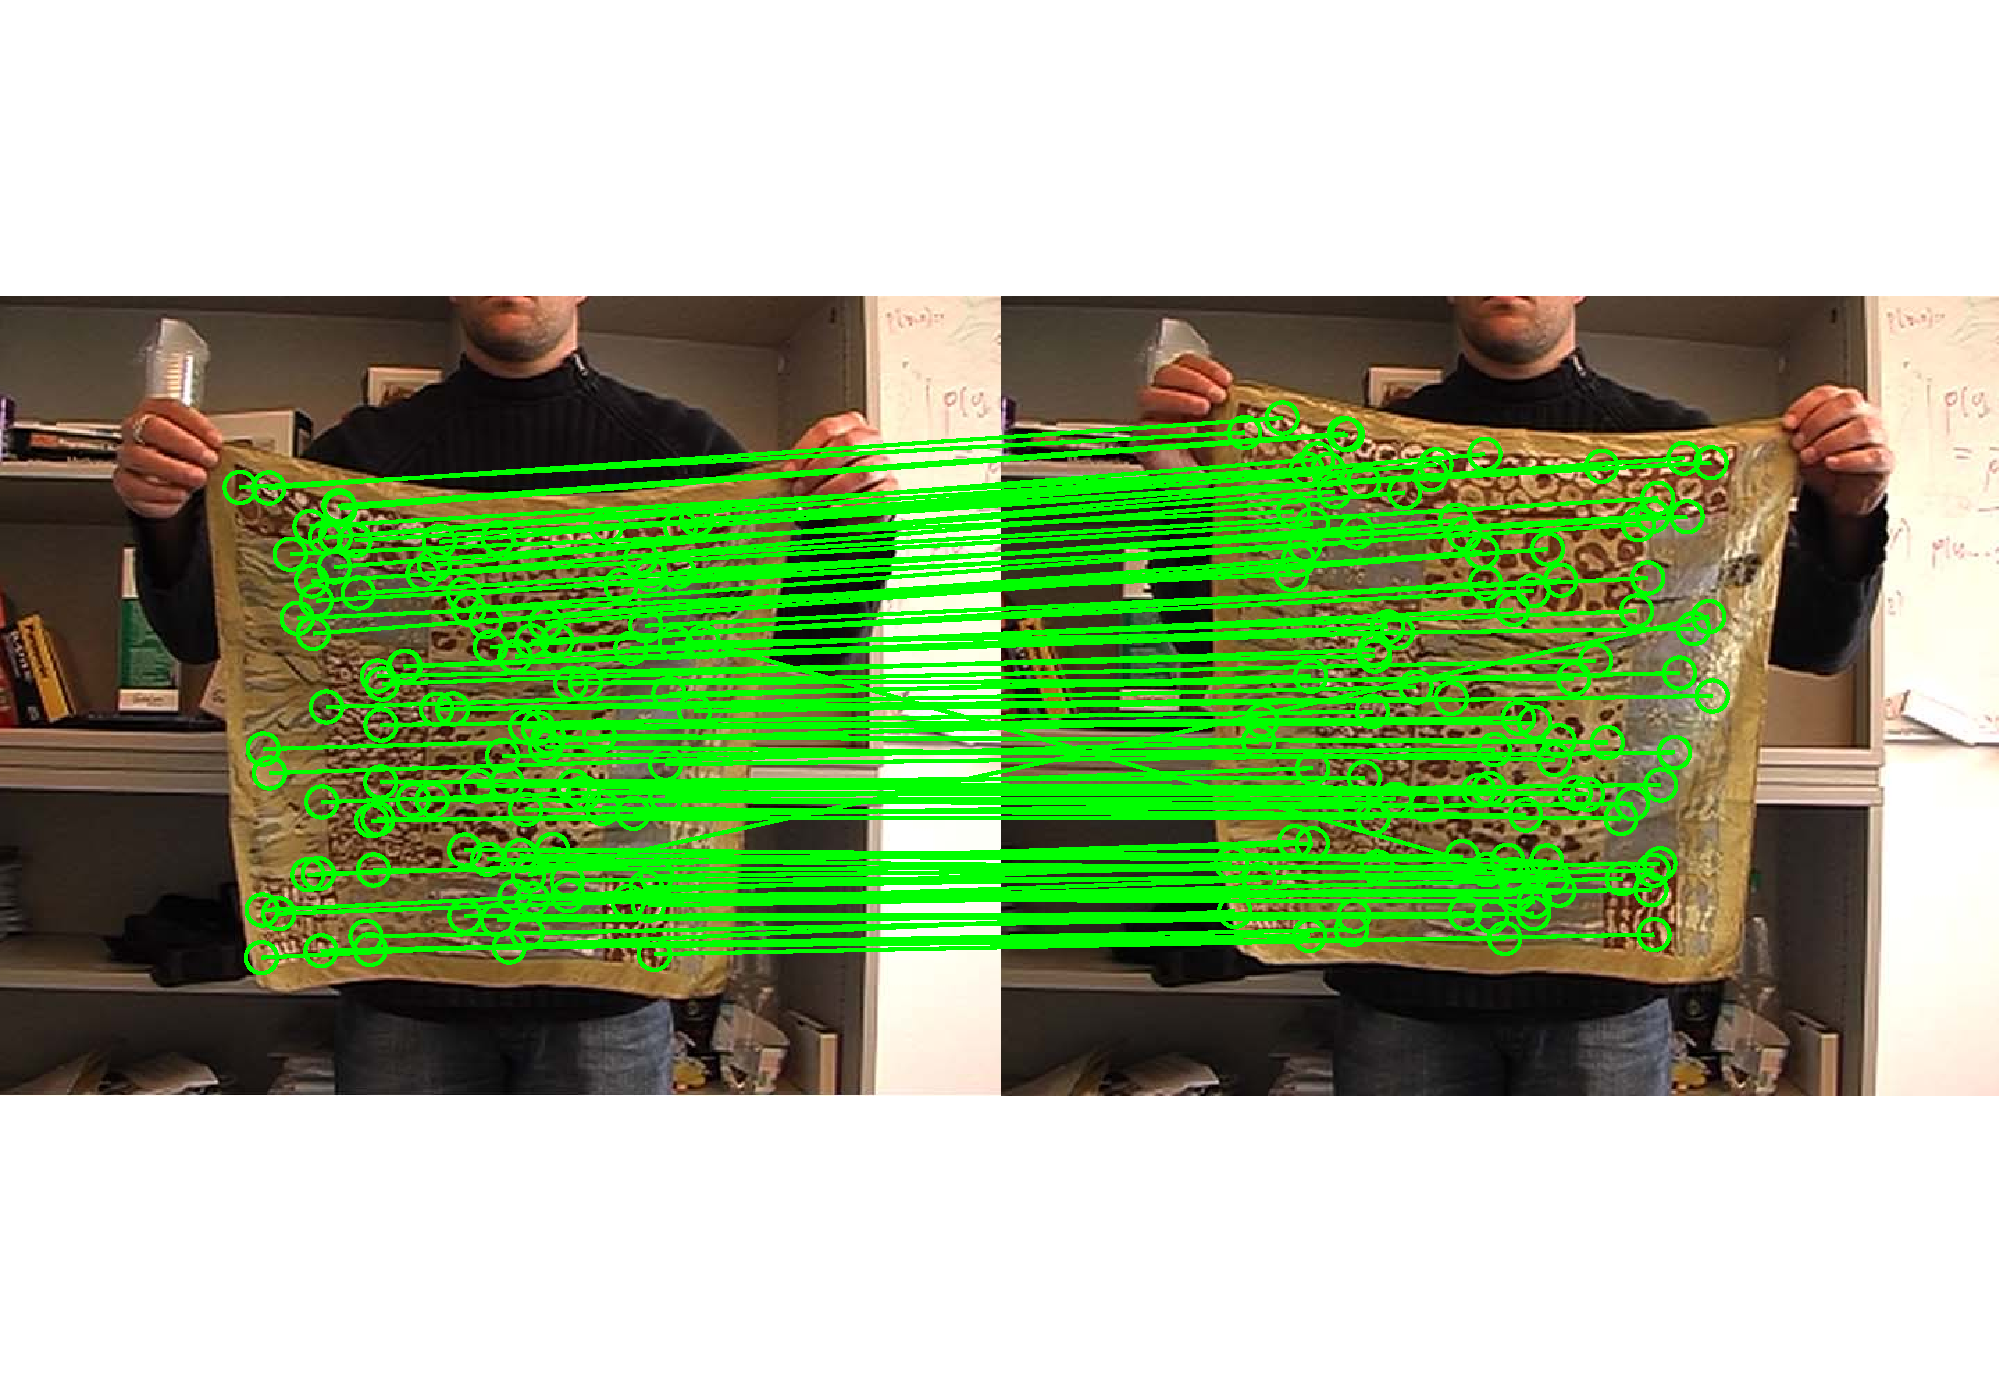
\includegraphics[width=62mm]{hyper_F258-F299.pdf}%
            }%
        \end{minipage}%
        \hspace{10mm}%
        \addtocounter{subfigure}{-1}%
        %%%
        \begin{minipage}[b]{0.4\textwidth}
        \subfigure{
            \label{fig:subfig:clothmatching4}
            \centering
            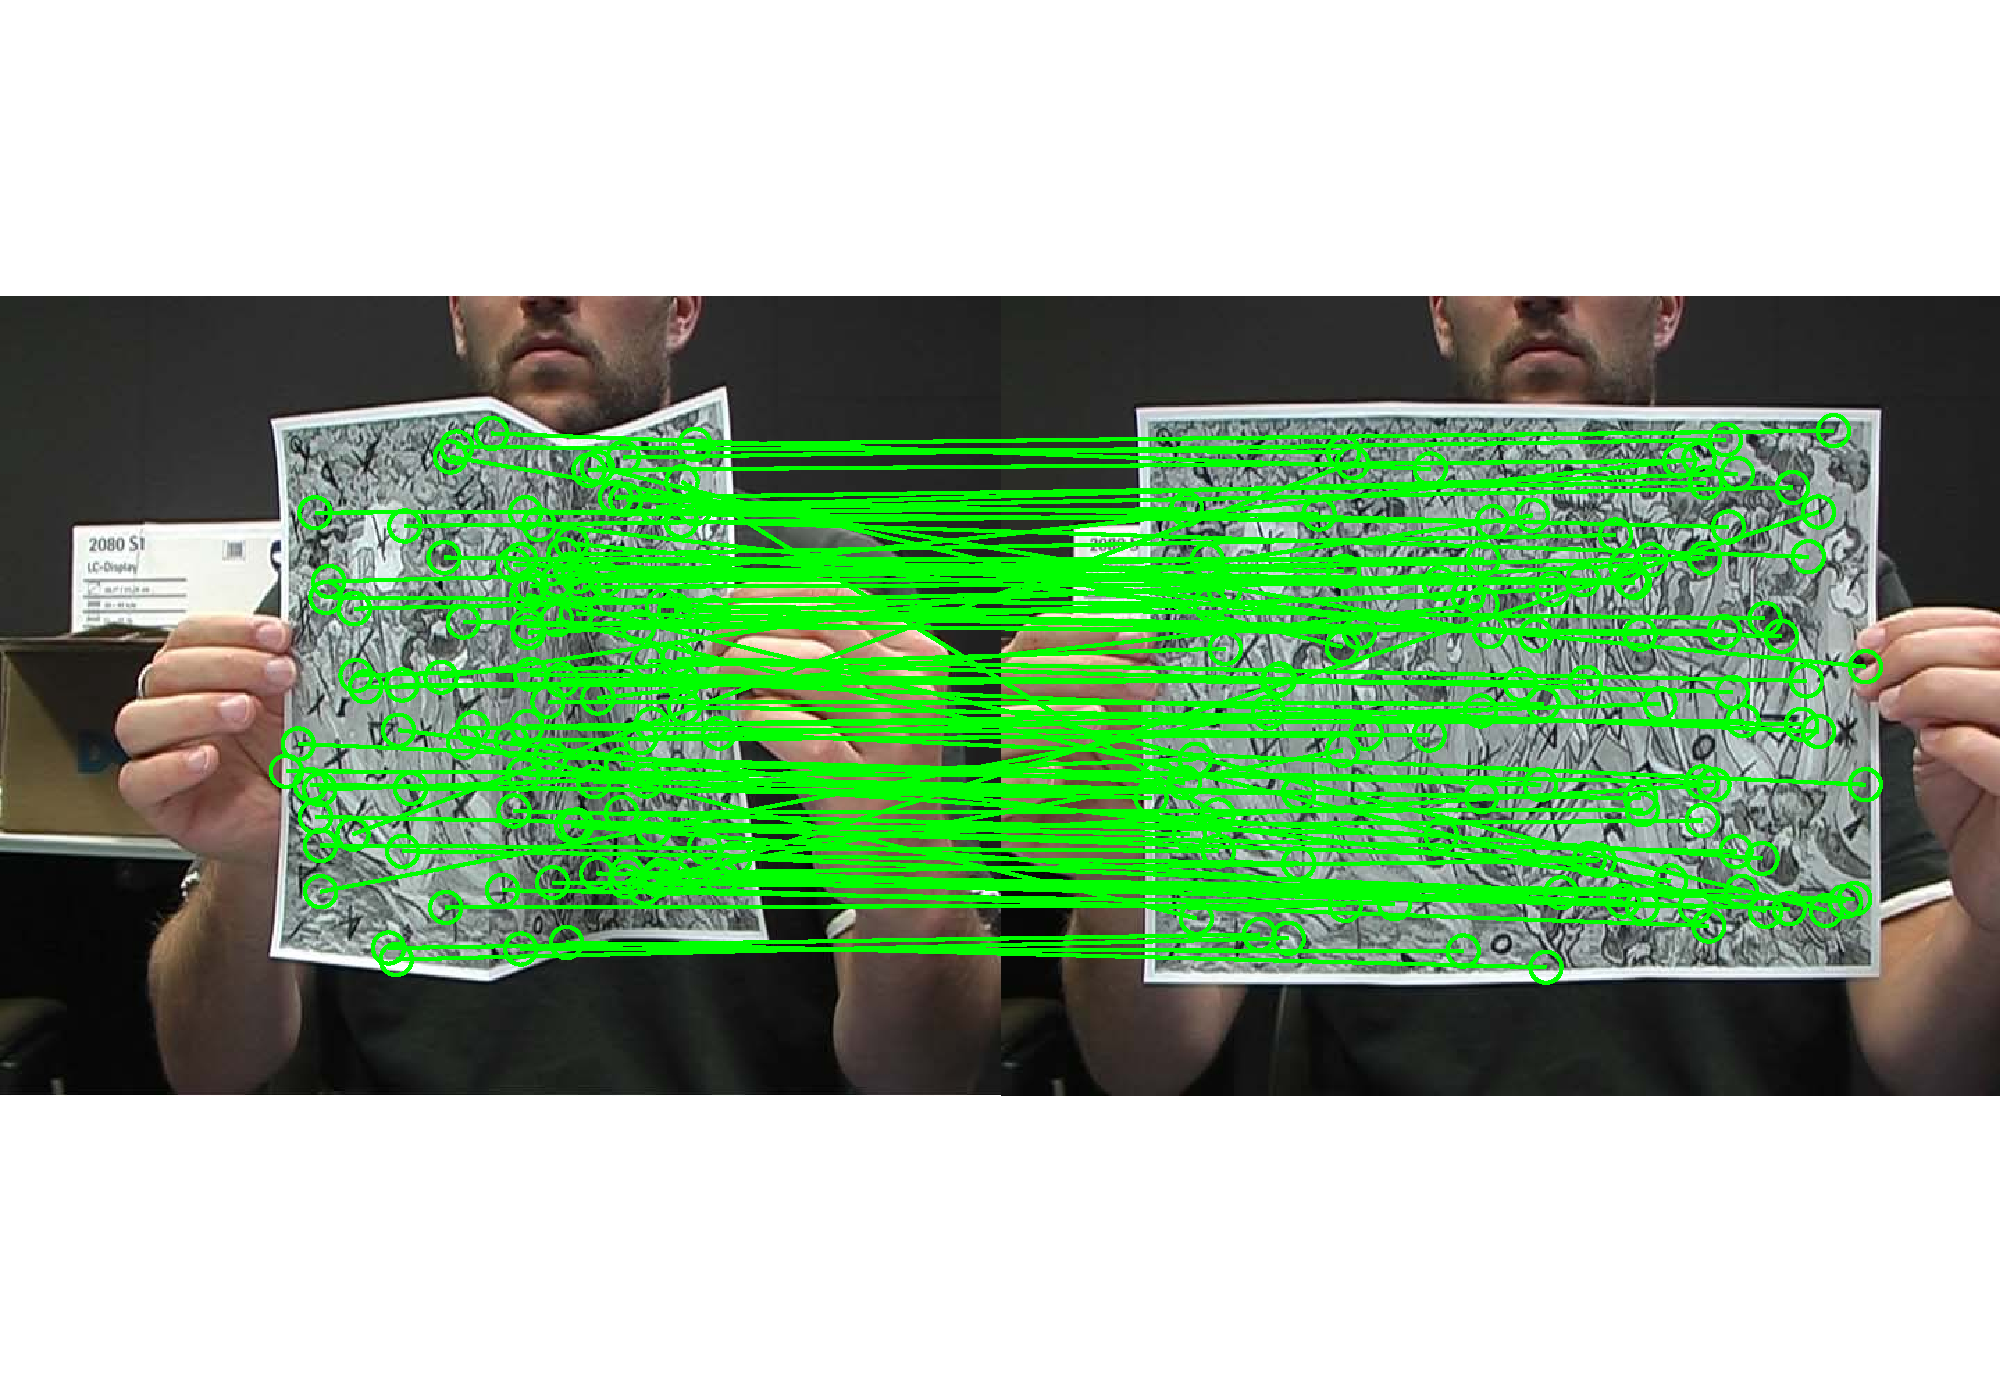
\includegraphics[width=60mm]{hyper_F309-375.pdf}%
            }%
        \end{minipage}\\%
        %\hspace{-16ex}%
        \addtocounter{subfigure}{-1}%
        %----------------------------
        %%% DEMO method
        %----------------------------
        \hspace{-8ex}
        \begin{minipage}[b]{0.4\textwidth}
        \subfigure{
            \label{fig:subfig:papercmatching1}
            \centering
            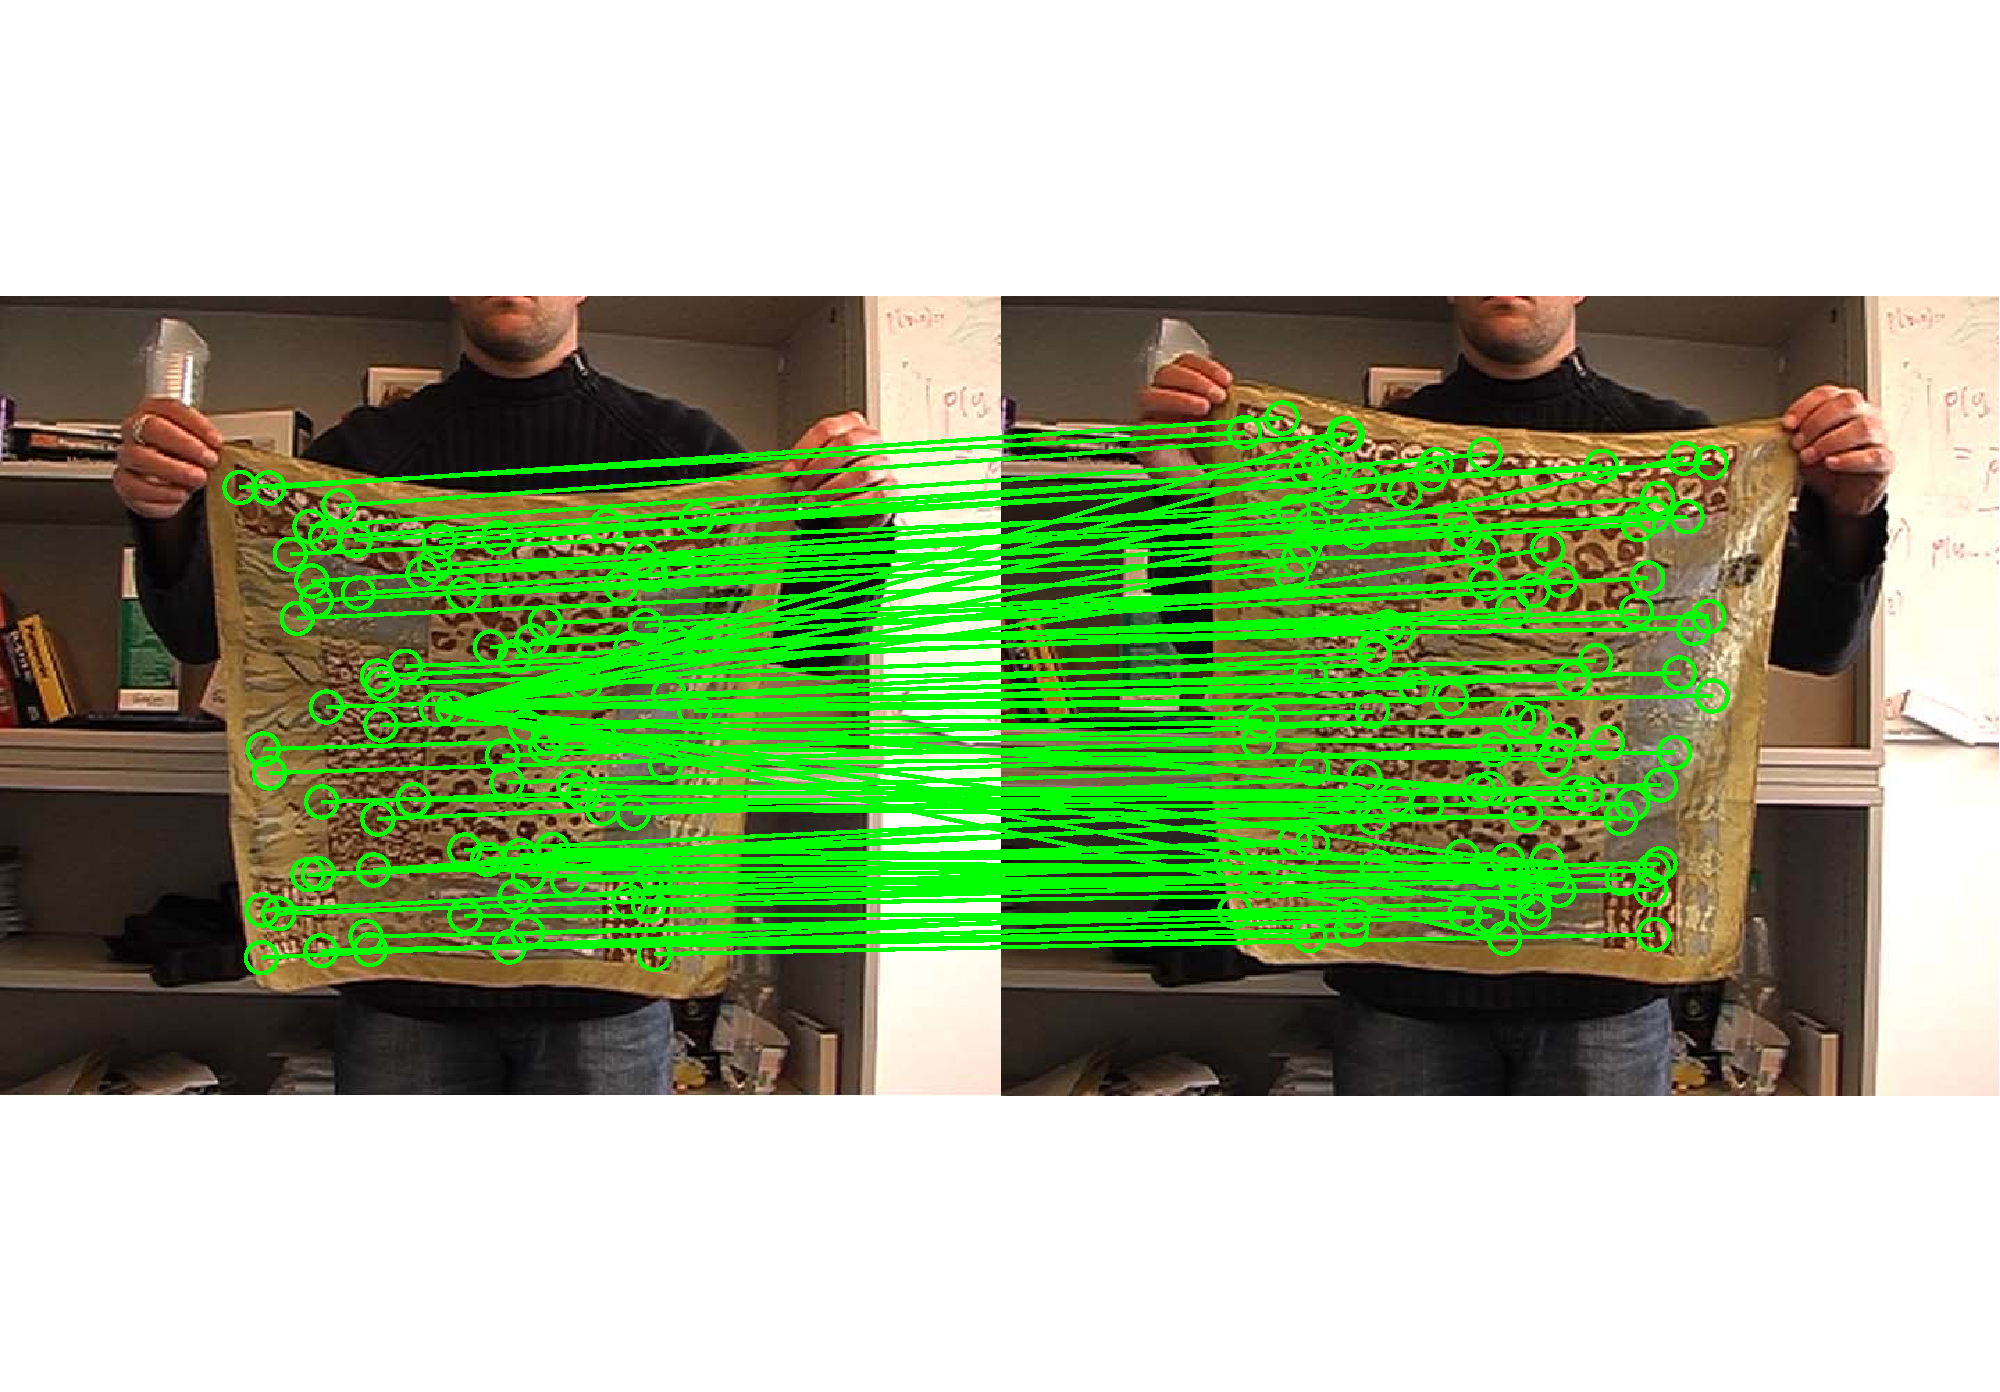
\includegraphics[width=62mm]{3demo_F258-F299.pdf}%
            }%
        \end{minipage}%
        \hspace{10mm}%
        \addtocounter{subfigure}{-1}%
        %%%
        \begin{minipage}[b]{0.4\textwidth}
        \subfigure{
            \label{fig:subfig:papercmatching2}
            \centering
            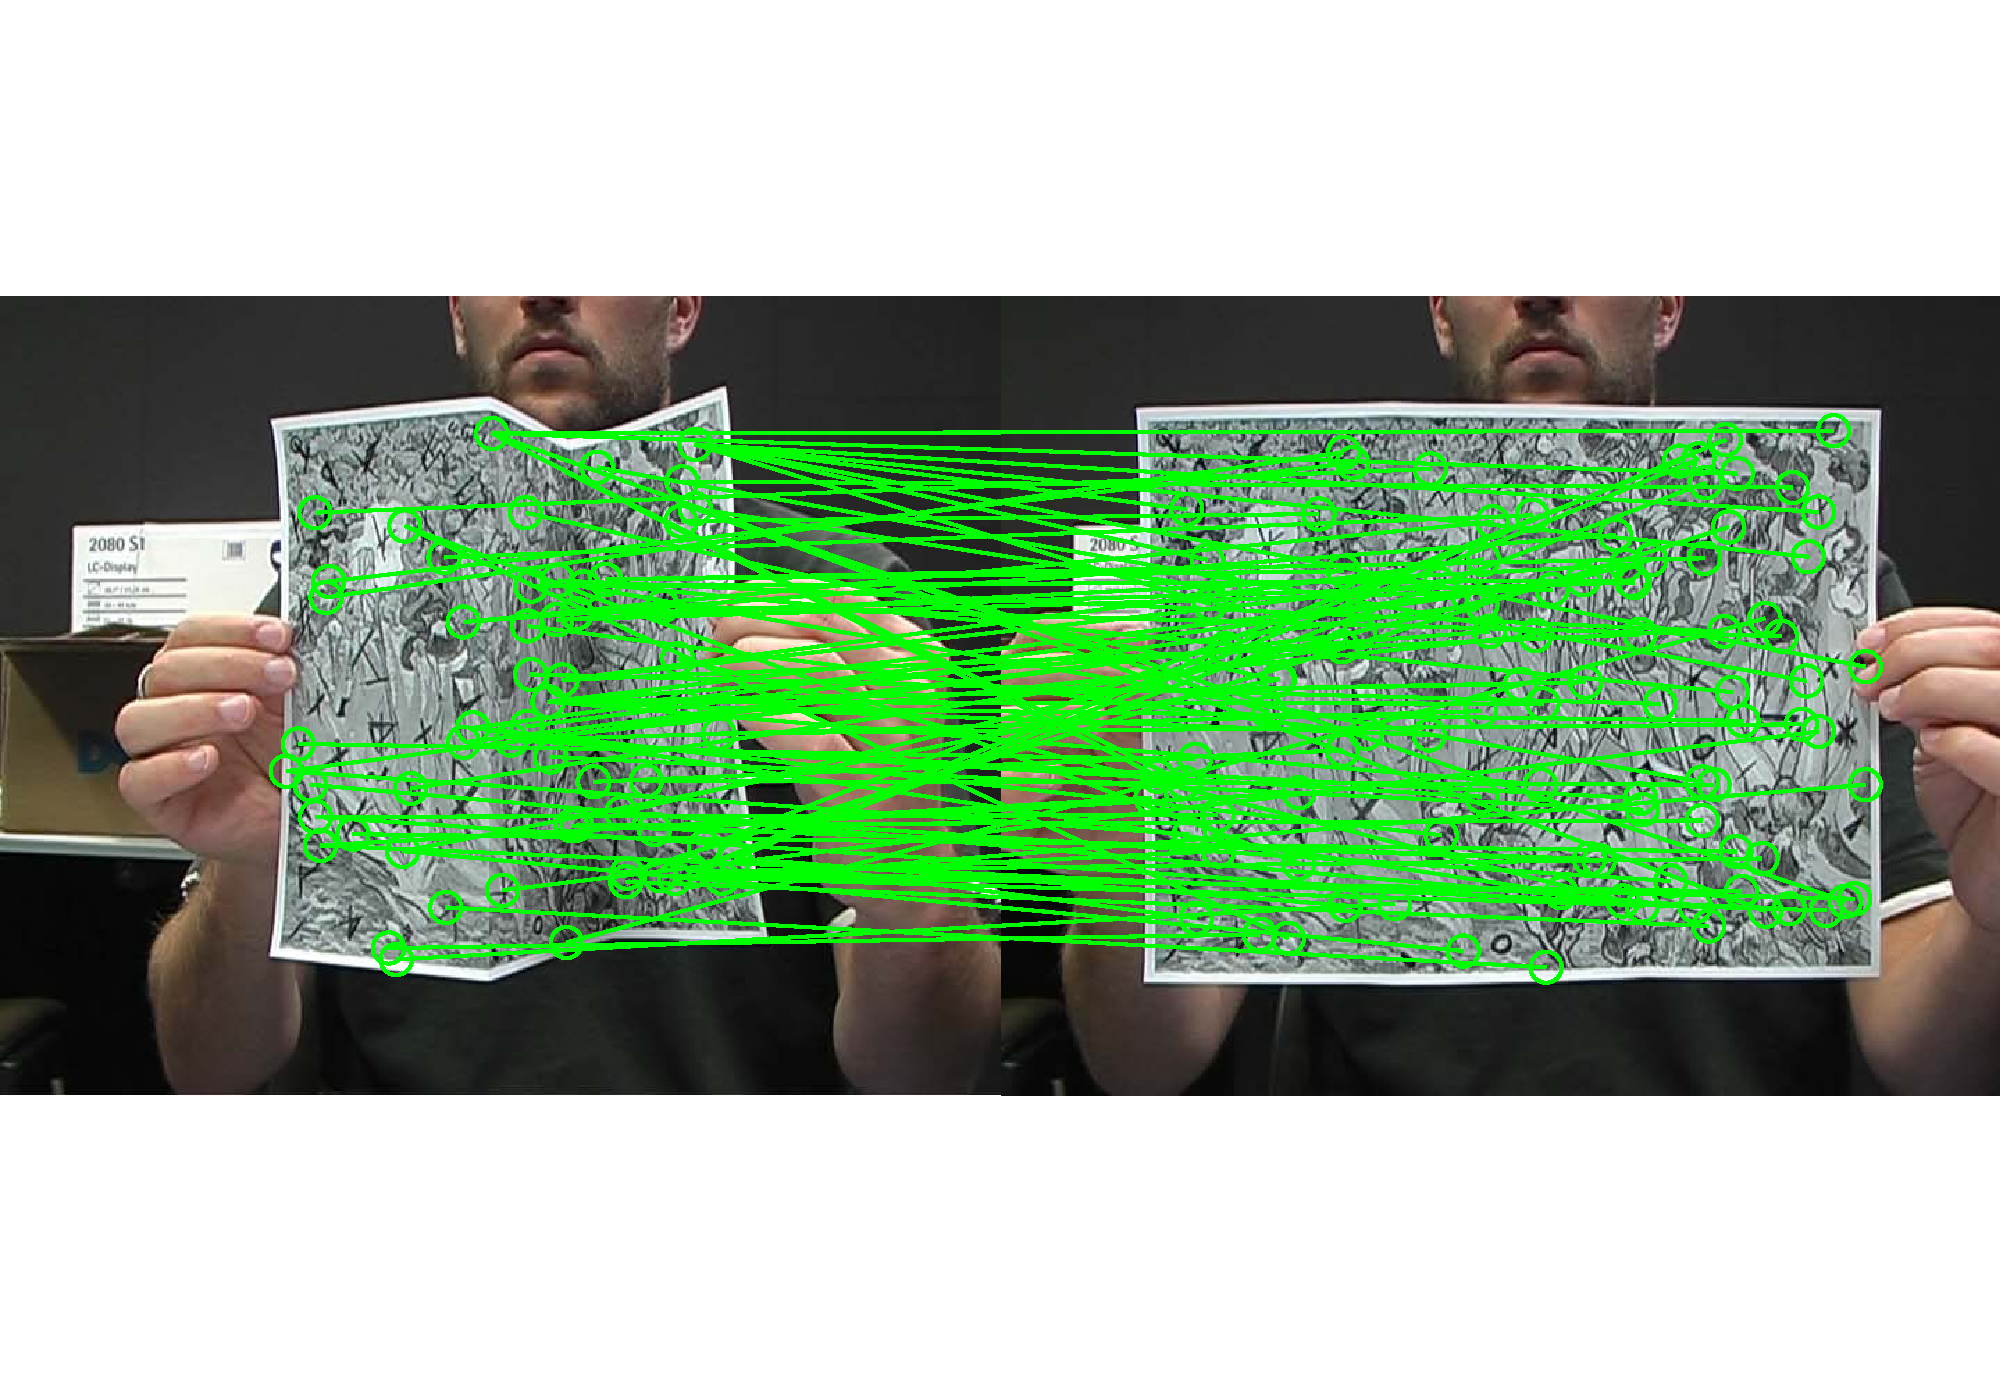
\includegraphics[width=60mm]{3demo_F309-375.pdf}%
            }%
        \end{minipage}\\%
        %\hspace{28mm}%
        \addtocounter{subfigure}{-1}%
        %----------------------------
        %%% OUR method
        %----------------------------
        \hspace{-8ex}
        \begin{minipage}[b]{0.4\textwidth}
        \subfigure[]{
            \label{fig:subfig:papercmatching3}
            \centering
            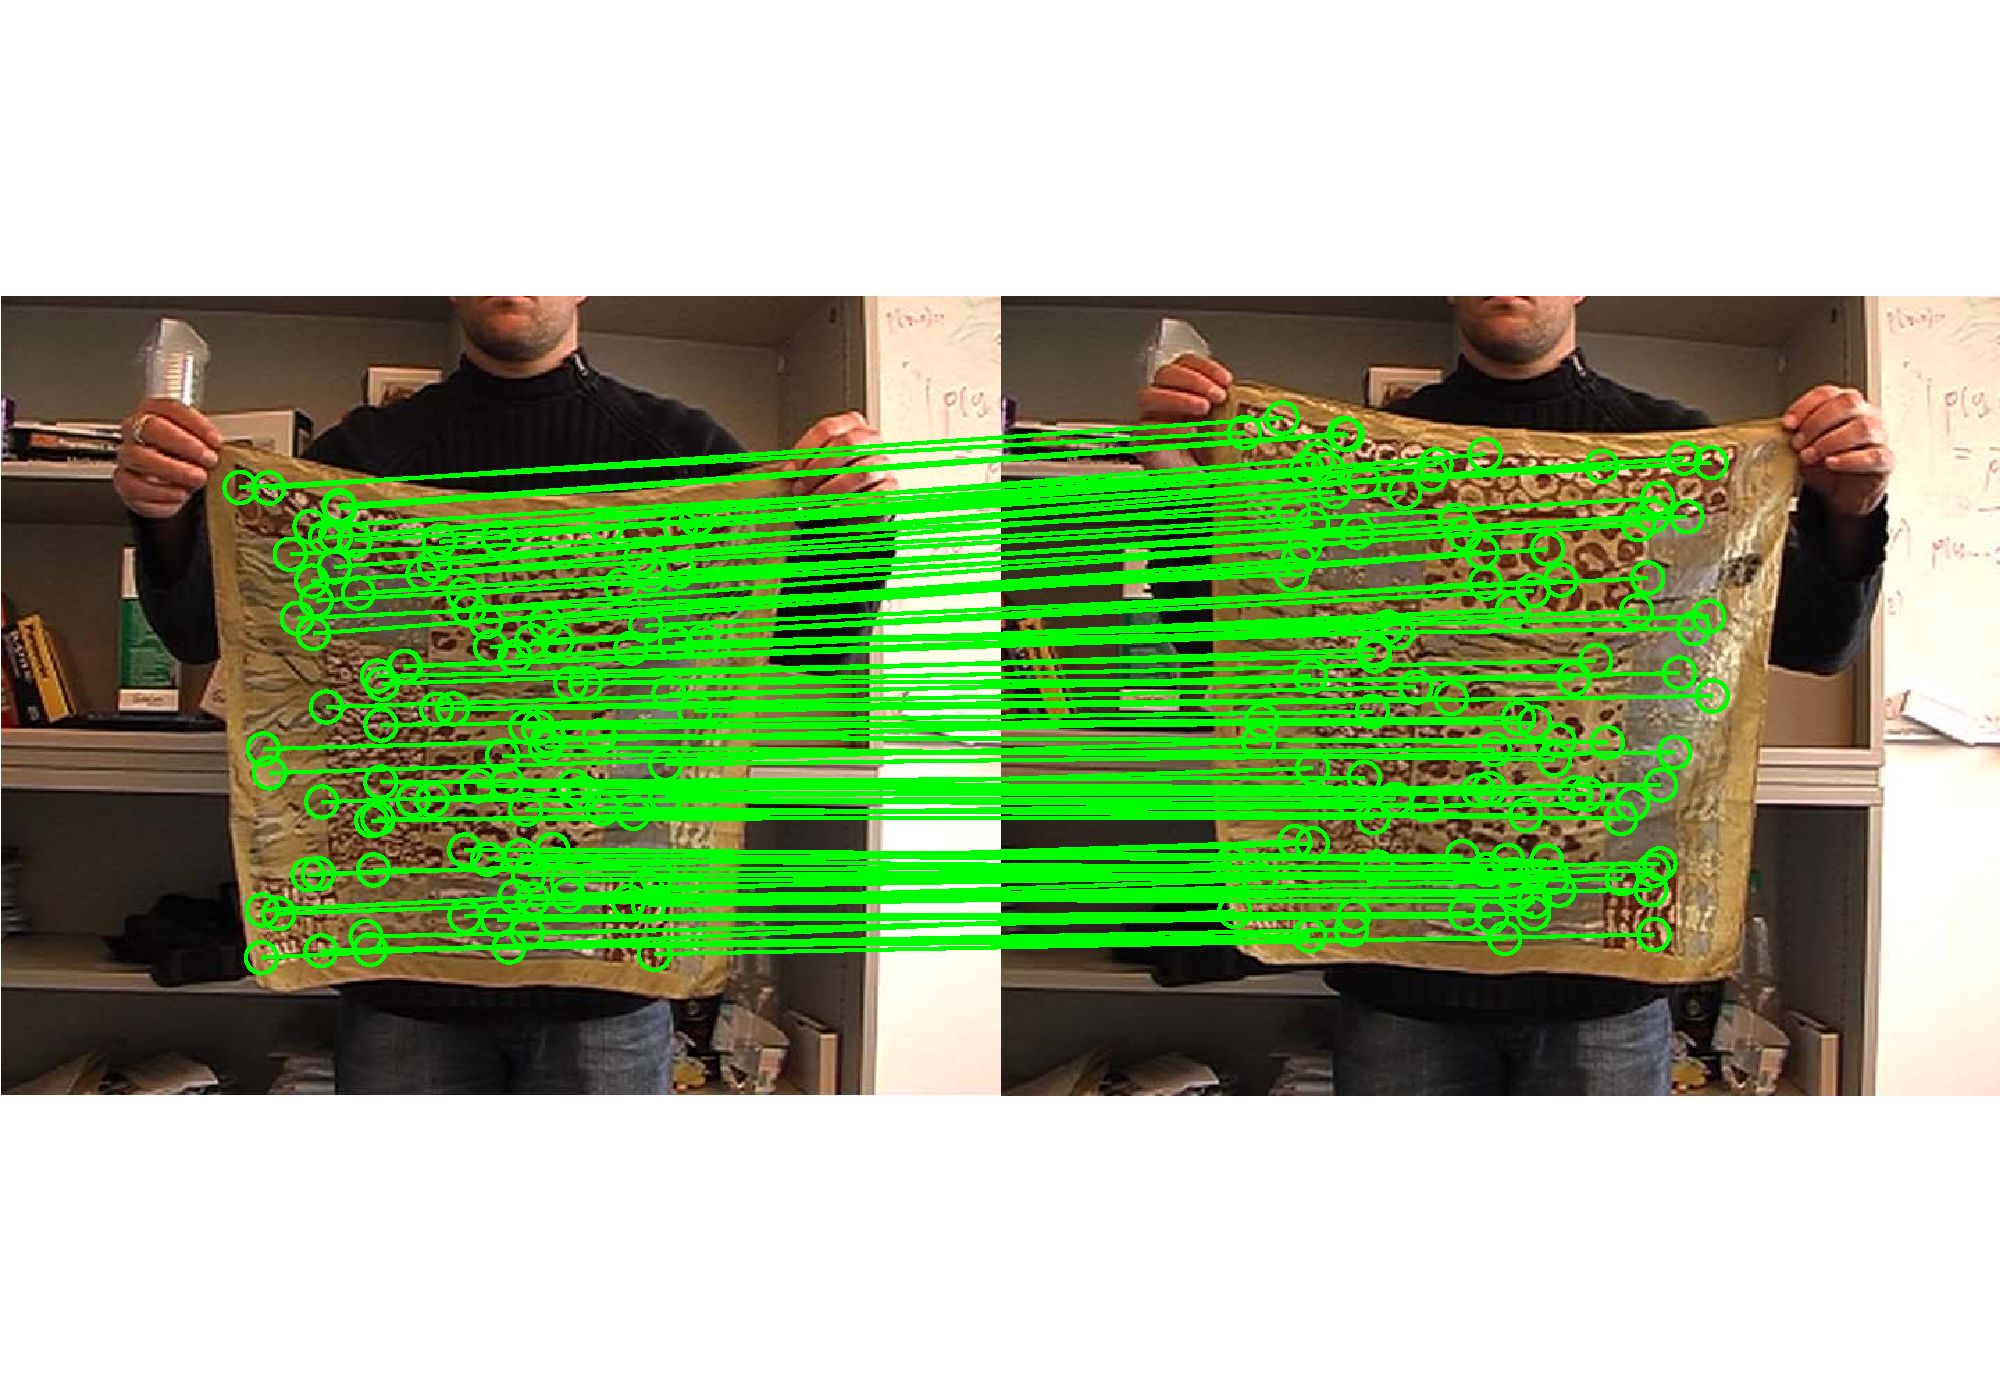
\includegraphics[width=60mm]{our_F258-F299.pdf}%
            }%
        \end{minipage}%
        \hspace{10mm}%
        %\addtocounter{subfigure}{-1}
        %%%
        \begin{minipage}[b]{0.4\textwidth}
        \subfigure[]{
            \label{fig:subfig:papercmatching4}
            \centering
            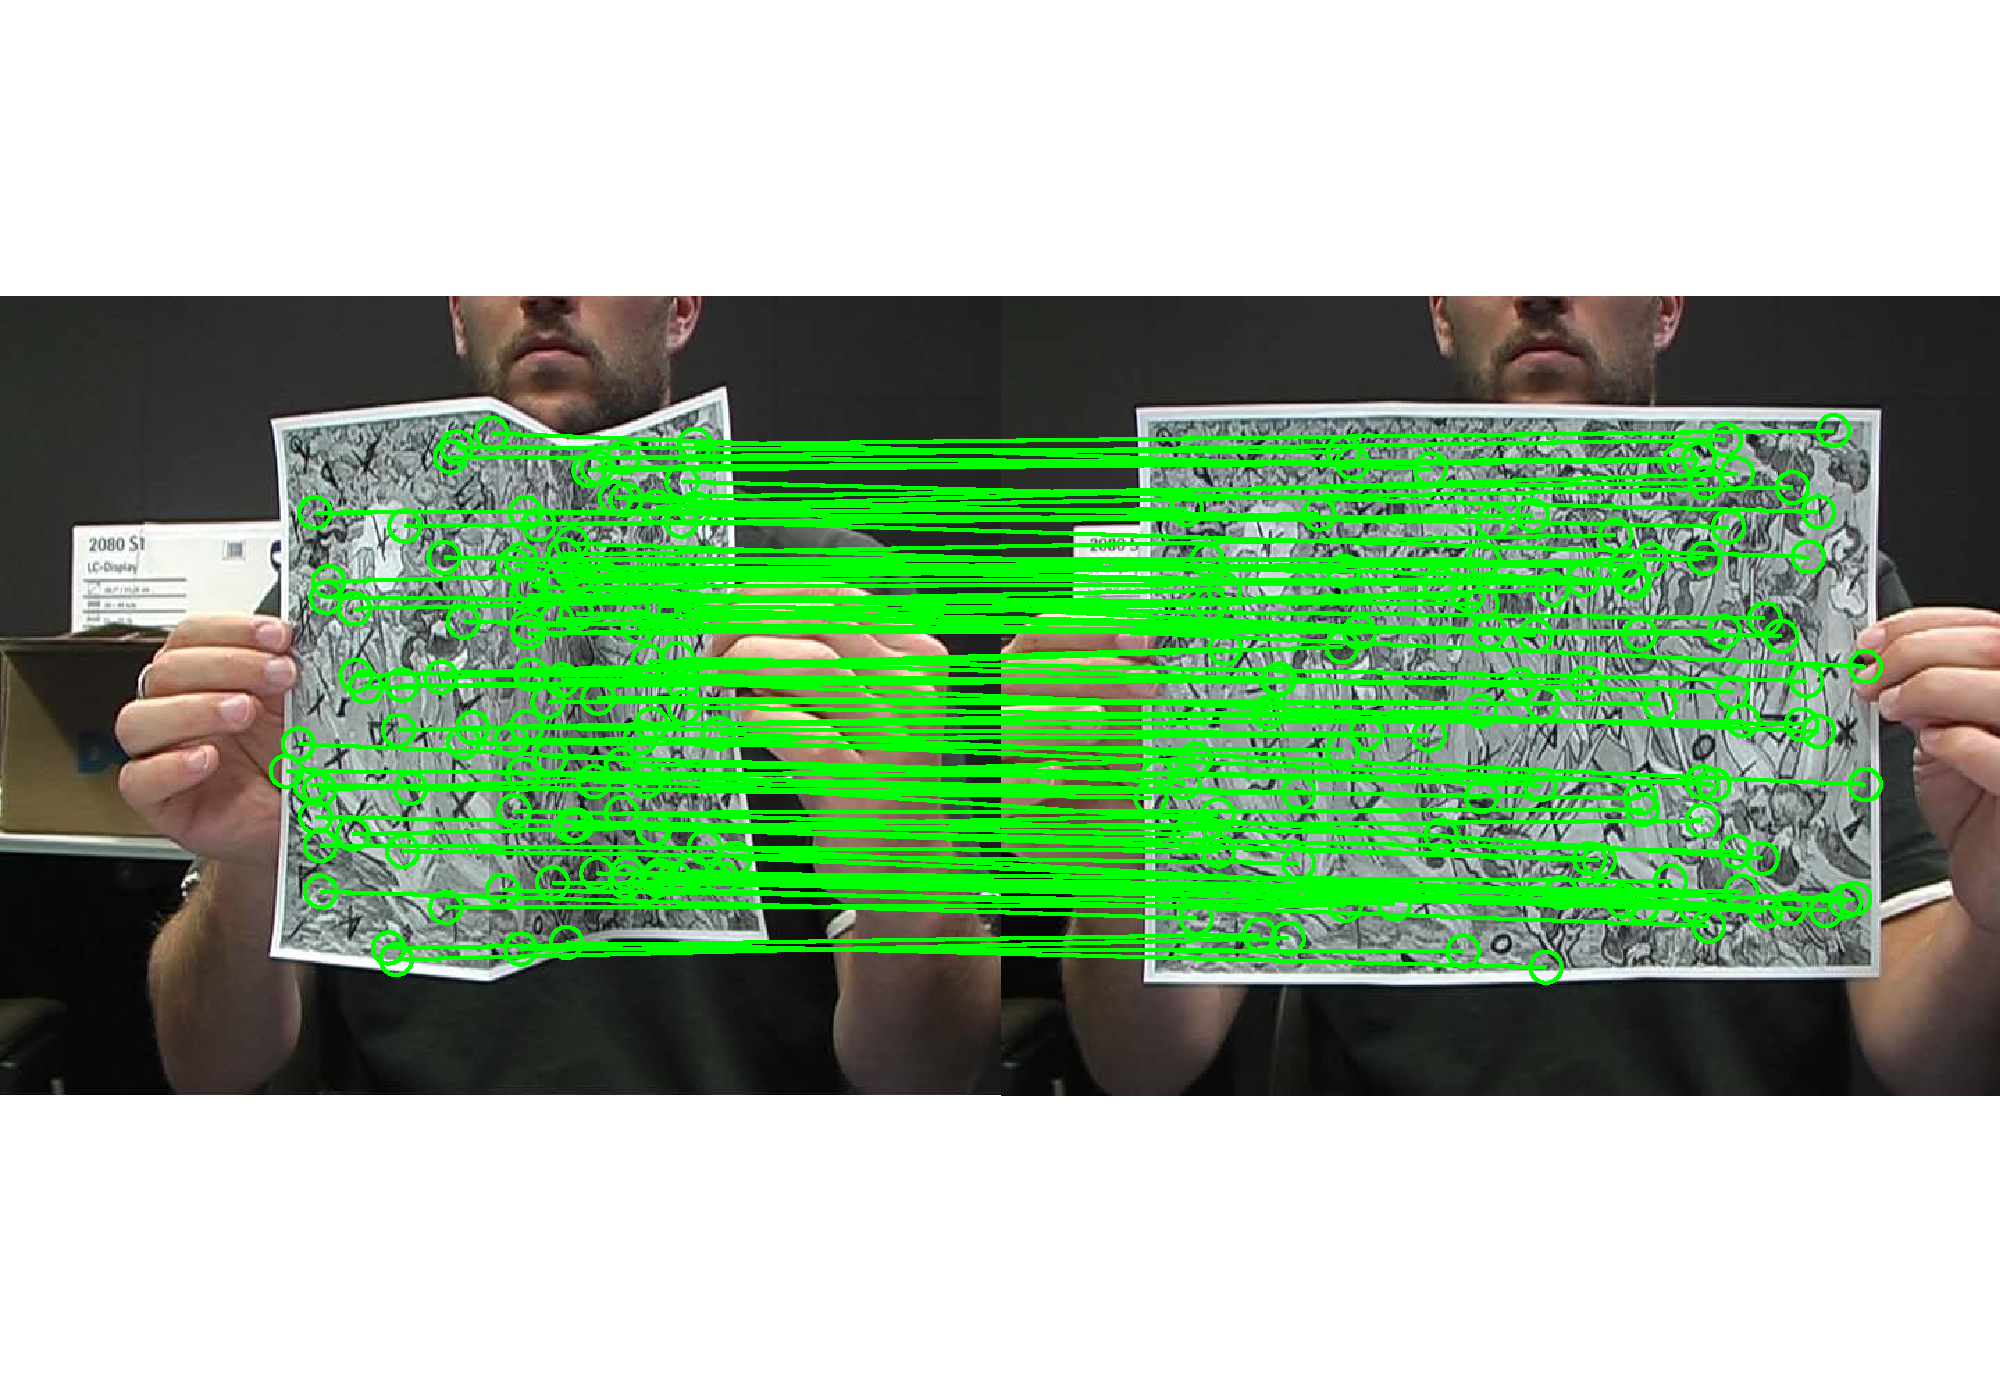
\includegraphics[width=60mm]{our_F309-375.pdf}%
            }%
        \end{minipage}%
        %\hspace{24mm}%
        %\addtocounter{subfigure}{-1}
        \caption{Matching results}
        %. Left: cloth set, frames 258 and299, right: creased paper set, frames 309 and 375. Top to bottom, spectral method~\cite{Cour06}, hyper graph matching method~\cite{Zass08}, a tensor based ~\cite{Duchenne09}, and our method.}
\label{fig:mini:deformablematchingimages} %% label for entire figure
%\vspace{-2ex}
\end{figure*}%
%----------------------------------------
%  deformable matching results TABLE
%----------------------------------------
\begin{table*}[!hp]
%\vspace{-4mm}
%\centering
\renewcommand{\arraystretch}{0.6}
\setlength{\aboverulesep}{0pt}
\setlength{\belowrulesep}{0pt}
\caption{Error rate of deformable surface matching.}
\hspace{-5ex}
\label{tab:errorrate1}
\begin{tabular}{c|c c c c c|c c c c c}
\toprule
\itshape \small{Dataset}  & \multicolumn{5}{|c|}{\itshape \small{cloth}}  & \multicolumn{5}{c}{\itshape \small{bending paper}} \\
\hline
\itshape \small{Matching} & \itshape \footnotesize{F88-}	& \itshape \footnotesize{F107-}	& \itshape\footnotesize{F120-}	& \itshape\footnotesize{F258-} & \itshape\footnotesize{F305-} & \itshape\footnotesize{F262-}	& \itshape\footnotesize{F275-}	& \itshape\footnotesize{F280-} & \itshape\footnotesize{F289-}	& \itshape\footnotesize{F301-}  \\
\itshape \small{frames}   & \itshape \footnotesize{F299}     & \itshape \footnotesize{F299}   & \itshape \footnotesize{F299}   &                \itshape \footnotesize{F299}  & \itshape \footnotesize{F299}  & \itshape\footnotesize{F314}    & \itshape \footnotesize{F314}   &                \itshape \footnotesize{F314}  & \itshape \footnotesize{F314}   & \itshape \footnotesize{F314} \\
\hline
\itshape \small{Our method} & \footnotesize 0	& \footnotesize 0	    & \footnotesize 0	    & \footnotesize 0	    & \footnotesize 0	  & \footnotesize0	        & \footnotesize 0	    & \footnotesize 0	    & \footnotesize 0	    &  \footnotesize 0  \\
%\hline
\itshape \small{\cite{Zass08}} &	 \footnotesize{2\%}	& \footnotesize{2\%}	&  \footnotesize{2\%}	& \footnotesize{2\%}	& \footnotesize{2\%} & \footnotesize{23\%}	 &  \footnotesize{9\%}	 & \footnotesize{23\%}	& \footnotesize{18\%}	& \footnotesize{14\%}  \\
%\hline
\itshape \small{\cite{Duchenne09}} & \footnotesize{25\%} & \footnotesize{41\%}   & \footnotesize{30\%}	& \footnotesize{30\%}	 & \footnotesize{42\%}	& \footnotesize{71\%}	 & \footnotesize{67\%}	& \footnotesize{59\%}	& \footnotesize{55\%}	& \footnotesize{50\%}  \\
%\hline
\itshape \small{\cite{Cour06}}      & \footnotesize{93\%} & \footnotesize{83\%}	&  \footnotesize{77\%}	&  \footnotesize{94\%}	& \footnotesize{90\%}	 & \footnotesize{93\%}	 & \footnotesize{98\%}	 & \footnotesize{99\%}	& \footnotesize{93\%}	& \footnotesize{96\%}  \\
\bottomrule
\end{tabular}%
%\vspace{-27pt}
%\vspace{-8mm}
\end{table*}%
%
\begin{table*}[!htbp]
%\vspace{-15pt}
%\centering
\renewcommand{\arraystretch}{0.6}
\setlength{\aboverulesep}{0pt}
\setlength{\belowrulesep}{0pt}
\caption{Error rate of deformable surface matching.}
\label{tab:errorrate2}
\hspace{-5ex}
\begin{tabular}{c|c c c c c|c c c c c}
\toprule
\itshape \small{Dataset}  & \multicolumn{5}{|c|}{\itshape \small{cushion}}  & \multicolumn{5}{c}{\itshape \small{creased paper}} \\
\hline
\itshape \small{Matching} & \itshape \footnotesize{F144-}	& \itshape \footnotesize{F156-}	& \itshape\footnotesize{F165-}	& \itshape\footnotesize{F172-} & \itshape\footnotesize{F188-} & \itshape\footnotesize{F309-}	& \itshape\footnotesize{F320-}	& \itshape\footnotesize{F330-} & \itshape\footnotesize{F340-}	& \itshape\footnotesize{F352-}  \\
\itshape \small{frames}   & \itshape \footnotesize{F213}     & \itshape \footnotesize{F213}   & \itshape \footnotesize{F213}   &                \itshape \footnotesize{F213}  & \itshape \footnotesize{F213}  & \itshape\footnotesize{F375}    & \itshape \footnotesize{F375}   &                \itshape \footnotesize{F375}  & \itshape \footnotesize{F375}   & \itshape \footnotesize{F375} \\
\hline
\itshape \small{Our method} & \footnotesize 0	& \footnotesize 0	    & \footnotesize 0	    & \footnotesize 0	    & \footnotesize 0	  & \footnotesize0	        & \footnotesize 0	    & \footnotesize 0	    & \footnotesize 0	    &  \footnotesize 0  \\
%\hline
\itshape \small{\cite{Zass08}} &	 \footnotesize{8\%}	& \footnotesize{10\%}	&  \footnotesize{2\%}	& \footnotesize{6\%}	& \footnotesize{5\%} & \footnotesize{22\%}	 &  \footnotesize{10\%}	 & \footnotesize{11\%}	& \footnotesize{2\%}	& \footnotesize{6\%}  \\
%\hline
\itshape \small{\cite{Duchenne09}} & \footnotesize{61\%} & \footnotesize{65\%}   & \footnotesize{59\%}	& \footnotesize{49\%}	 & \footnotesize{30\%}	& \footnotesize{80\%}	 & \footnotesize{74\%}	& \footnotesize{77\%}	& \footnotesize{68\%}	& \footnotesize{46\%}  \\
%\hline
\itshape \small{\cite{Cour06}}      & \footnotesize{95\%} & \footnotesize{92\%}	&  \footnotesize{93\%}	&  \footnotesize{93\%}	& \footnotesize{92\%}	 & \footnotesize{98\%}	 & \footnotesize{94\%}	 & \footnotesize{96\%}	& \footnotesize{92\%}	& \footnotesize{88\%}  \\
\bottomrule
\end{tabular}%
%\vspace{10pt}
\end{table*}%

%-------------------------------------------------------------------------
\subsection{3D rigid object scans}
\label{subsec:3drigid}

%-------------------------------------------------------------------------
\subsection{3D articulated object scans}
\label{subsec:3darticulated}

%-------------------------------------------------------------------------
\subsection{3D colorful object scans}
\label{subsec:3dColored}
